\documentclass[12pt,a4paper]{article}

\usepackage[T1]{fontenc}
\usepackage[utf8]{inputenc}
\usepackage[english]{babel}
\usepackage{lmodern}
\usepackage{geometry}
\usepackage{setspace}
\usepackage{amsmath,amssymb}
\usepackage{booktabs}
\usepackage{graphicx}
\graphicspath{{./}{figuras/}}
\usepackage{tabularx}
\usepackage{hyperref}
\usepackage{natbib}
\usepackage{csquotes}
\usepackage{float}
\usepackage{caption}
\usepackage{enumitem}
\usepackage{multirow}

\geometry{margin=2.5cm}
\onehalfspacing
\hypersetup{colorlinks=true,linkcolor=black,citecolor=black,urlcolor=blue}

\title{Gradual payroll re-taxation and the formal labor market:\\evidence from Law no.\ 14.973/2024}
\author{Victor Moreschi}
\date{October 2026}

\begin{document}
\maketitle

\begin{abstract}
\noindent
We examine the effect on formal employment, in the short run, of the exit from the payroll-tax relief under Law 14.973/2024, which, starting in 2025, reinstated the payroll contribution for activity classes listed in articles 7 and 8 of Law 12.546, in two steps (in 2025 and in the first half of 2026, 5\% and 10\%, respectively), while the rate for the classes in the same CNAE sections that were not listed remained at 20\%. The statute sets the dose (0, 5 and 10) in a difference-in-differences setup. Saturating the dose with two year effects, $\beta_5$ and $\beta_{10}$, relative to the 2023--24 base, and using Novo CAGED data up to June 2026, we find $\hat\beta_5 = 0.020$ [$-0.064$; $0.104$] and $\hat\beta_{10} = 0.011$ [$-0.11$; $0.13$] (coefficient and 95\% CI), for net employment, small and not statistically significant, but the CIs are wide relative to the cell-month mean of 0.30 and cannot rule out large effects. Under strong parallel trends, $(\beta_{10}-\beta_5)/5$ would be the average causal response of the increase from 5 to 10; because the same classes move from dose 5 to dose 10, it may be confounded by dynamic effects and class-specific shocks. Using 2023 leads as a plausibility check relative to the 2024 base, we do not reject the parallel trends hypothesis for net employment with the studentized maximum test in the full sample, but we reject when we drop construction.
\end{abstract}
\noindent\textit{Keywords:} payroll re-taxation; difference-in-differences; continuous treatment; CAGED; formal employment.

\noindent\JEL{JEL classifications: J23, H25, J32, H55}
% =====================================================================
\section{Introduction}

Employers hiring formal workers pay a social security tax of 20 percent on payroll in Brazil. From 2011, a number of labor-intensive sectors paid a social security contribution on gross revenue, ranging from 1\% to 4.5\% of revenue, instead of the 20\% of payroll, in an attempt to reduce the relative cost of formal hiring (Law 12.546). On September 16, 2024, Law 14.973 was sanctioned and published. It established a phase-in of the 20 percent payroll rate for these sectors, by charging 5 percent of payroll in 2025, 10 percent in 2026, 15 percent in 2027, and 20 percent starting in 2028, at which point the contribution on revenue will be extinguished.

Did the higher cost of formally employing workers in the re-taxed classes change net formal employment (hires minus separations), relative to sectors that already paid 20\%? Hires, separations and starting wages are analyzed in the same specification. For the period of relief (2013-2018 and 2018-2024), the estimates on employment are very weak (or null) \citep{reckziegel2024, albernaz2025}.

This paper considers the exit from the relief, from 2025 on. The classes established in articles 7 and 8 of the Law 12.546 started to pay the payroll tax again from January of that year. On the other hand, other classes in the same CNAE section, never listed in articles 7 and 8, kept paying 20\%. This allows the comparison of the evolution of formal firms outside the Simples that operate in related activities.

Firms could follow the hybrid path only if their average employment over the calendar year stayed at least 75\% of the previous year's average; otherwise they would be subject to the full 20\% rate. Because net employment is the change in the stock, this rule limits large net separations, but it does not constrain hires and separations that offset each other (Section 2).

This setting suggests a difference-in-differences with continuous treatment, as in \citet{callaway2024}. But, differently from the usual setting in the literature, the dose takes discrete values in $\{0,5,10\}$. Then, the main specification for the coefficient on the dose is actually a saturation with two year effects, $\beta_{5}$ and $\beta_{10}$ for 2025 and 2026, relative to the base period in 2023-2024. The linear specification, that would be more standard in this setting, would impose a linearity that is not necessarily in the law. Moreover, the classes in the law that were supposed to be listed and those that were not may have different seasonality. Then, the main specification includes class$\times$calendar month, municipality$\times$civil month, class$\times$municipality$\times$calendar month and municipality$\times$year fixed effects. A leaner set of fixed effects (class $\times$ calendar month, municipality and civil month) and a linear specification in the dose are used for comparison. The preferred specification of the Event Study has the same FE as the preferred specification, and uses the interaction of the event time with a dose that was assigned for that purpose. The binary Event Study interacts the variable that indicates if the class was supposed to be listed in the law with the event time, with the same FE as the preferred specification. Under strong parallel trends in dose, the difference $\beta_{10}-\beta_5$, divided by 5, measures the average causal response to the step from 5 to 10. Because the same classes move from dose 5 to dose 10, this contrast also reflects dynamic effects and shocks specific to the listed classes between 2025 and 2026, and the 2023 leads are only a plausibility check on parallel trends.

The sections \ref{sec:contexto} and \ref{sec:dados} present the institutional context and the data used in the analysis. The sections \ref{sec:metodo} and \ref{sec:results} describe the methodology and the results. Robustness checks are presented in Section \ref{sec:robustness}. Section 6.5 presents sample cuts. Section 7 discusses the results and their limits, and Section 8 concludes. Supporting figures are in Appendices A--C.

\section{Institutional setting}
\label{sec:contexto}

Instead of paying 20\% of payroll, these firms paid 1\% to 4.5\% of gross revenue. At the beginning of the policy, the eligible activities, according to articles 7 and 8 of the Law \textbf{12.546/2011}, were: (i) clothing and apparel industry; (ii) footwear industry; (iii) textile industry; (iv) leather industry; (v) civil and infrastructure construction; (vi) call centers; (vii) information technology and ICT; (viii) integrated circuits design; (ix) communications; (x) animal protein; (xi) machinery and equipment industry; (xii) vehicle and body manufacturing industry; (xiii) freight road transport; and (xiv) urban passenger road transport and metro and urban rail passenger transport. There are 141 classes listed in the Law, however, not all of them were used in the estimation sample.

The policy was extended many times, and the Law \textbf{13.670/2018} excluded some subclasses. \cite{albernaz2025} studied the re-taxation of those activities and did not find any statistically relevant effect on their employment. The Law \textbf{14.784/2023} would have extended the relief through 2027. Its effects were suspended by an injunction in ADI 7633. Law \textbf{14.973/2024} replaced that arrangement with the hybrid ramp studied here.

\begin{table}[H]
\centering
\caption{Schedule under Law 14.973/2024}
\label{tab:cronograma}
\begin{tabular}{lcc}
\toprule
Year & Payroll contribution & Revenue contribution \\
\midrule
2024 & 0\% & full rate (1\% to 4.5\%) \\
2025 & 5\% & 80\% of the full rate \\
2026 & 10\% & 60\% of the full rate \\
2027 & 15\% & 40\% of the full rate \\
2028-- & 20\% & extinguished \\
\bottomrule
\end{tabular}
\end{table}

Note that this provision only applies to Lucro Real and Lucro Presumido companies. To stay in this transitional regime, the firm must maintain an average employment over the calendar year that is at least 75\% of the average employment over the previous calendar year. This requirement is based on the number of employees at the firm, not on retaining the same employees. Thus, a firm could separate an employee and hire a new employee and still be able to stay in the transitional regime. However, the firm’s ability to separate a large number of its employees on net is constrained because that would reduce the firm’s average employee stock. Between 2025 and 2027 the 13th salary is outside the transitional payroll contribution. That exemption applies only to firms on the transitional regime, so it is part of the treatment.
As discussed in Section \ref{sec:metodo}, the counterfactual are firms that are formally registered, not in Simples, and that would have the contribution rate on payroll unchanged in 2025. These are the classes not listed in articles 7 and 8 of Law 12.546. For example, in the manufacturing sector, the apparel industry is treated and the chemical industry, in the same section of apparel, is in the control group. For them, the contribution rate on payroll remained unchanged between 2024 and 2026, while for the classes listed in the law, it increased by 10 percentage points.

There is no way of telling apart the firms that chose the hybrid path from those that decided to go back to the full 20\% as the CNAE classification does not allow for it. Thus, the parameter of interest measures the intent to treat at the sectoral level.

The analysis is done until June 2026, the first year of dose 5 and first half of dose 10, since the law stipulates an increase to 15\% in 2027 and 20\% in 2028. As mentioned above, it is not possible to tell from the data which establishments chose to remain in the hybrid path and those that went back to 20\% within each class. Moreover, the establishment in the CAGED data are mixed with those in the Simples regime, which will also attenuate the effect of the policy at the sectoral level.

Since all classes are listed at the same time, there is no concern about staggered adoption and negative weights \citep{goodman2021using, de2022using}. However, there can be a difference in the seasonality of the calendar between classes that were listed in the law and those that were never listed. Thus, the main specification will use class$\times$calendar month, municipality$\times$civil month, class$\times$municipality$\times$calendar month and municipality$\times$year fixed effects, as described in Section \ref{sec:metodo}.

The contrast $(\beta_{10}-\beta_5)/5$ and its interpretation are discussed in Section 4.3.

\section{Data}
\label{sec:dados}

Novo CAGED micro (Jan'23 -- Jun'26). The raw data contain one row for each movement (hiring or separation), and report the class, municipality, contractual wage and type of movement. We aggregate the data to the class x municipality x month level (e.g., apparel industry in Campinas in Mar'25). Note that the CAGED only records a row if there was a movement, i.e., lack of a row means zero flow in that month. We thus fill in zeros for each class x municipality that was observed for at least one month over the 42 months.

We aggregate to the class x municipality x month level, and construct (i) net employment (our main outcome, the difference between hires and separations), (ii) hires, (iii) separations and (iv) the log of the average contractual wage of hires in each class x municipality in each month.

Time Period: 42 months. We start with 141 classes listed in the law, but drop four classes related to fishing (0311, 0312, 0321 and 0322) from our base set of classes. We then construct a set of control classes by including all classes in the same section as the treated classes; sections that do not contain any comparable classes, most notably public administration (Section O) and agriculture (Section A), are thus excluded from our analysis. In total, our estimation sample includes 137 treated classes and 248 control classes. In our principal specification, this gives a sample of $N=9{,}219{,}210$ cells for the flow outcomes (corresponding to 219,548 class x municipality pairs). In our leaner specification, we have a sample of $N=9{,}221{,}016$ for the flow outcomes.


Contractual wages outside 0.3 to 150 times the minimum wage are dropped, as are cells with at most two hires and a mean contractual wage above R\$\,50{,}000. August and September 2023 are dropped from the wage analysis only. In our principal specification, this gives a sample of $N=2{,}222{,}824$ for the wage outcome; in our leaner specification, a sample of $N=2{,}799{,}714$. In both specifications, the wage sample differs from the 2,799,760 wage cells in Table~\ref{tab:desc} only by singleton cells dropped by the fixed effects (576,936 in the principal specification, 46 in the leaner one). The wage filter drops contractual outliers. The cell rule is applied before the fixed effects, so it is already reflected in the $2{,}799{,}760$ wage cells. It drops thin cells whose mean contractual wage is not a usable hire wage. Aug'23 and Sep'23 are a data-quality episode in the contractual-wage file. The joint Wald test on the 2023 leads remains borderline for wages after that drop ($p\approx0.053$; Section 6.2). For the flow outcomes, we use the full panel.

\subsection{Raw descriptives}
\label{sec:desc}

Table~\ref{tab:desc} reports descriptive statistics for the classes included in the estimation sample. The completed panel contains 137 listed classes and 248 control classes. The full sample is therefore composed of 385 classes, 219,548 class$\times$municipality pairs, and 9,221,016 flow cells, of which 3,416,532 cells are listed. The gap between the number of flow cells in the estimation sample (9,219,210) and the full sample is due to flow cells that are dropped due to the inclusion of the saturated set of fixed effects in the main regression.

Before comparing mean net job flows, Table~\ref{tab:desc} also reports average hires and separations for each sample. Listed flow cells experience more hiring (5.65) and separations (5.35) per month on average than non-listed ones (4.11 and 3.84). Table~\ref{tab:desc} also reports the mean of the log starting wages for listed (7.65) and control (7.57) classes across the whole window, calculated over 1,083,678 and 1,716,082 wage cells respectively. Figure \ref{fig:raw_means} reports the raw means of net employment and of hires over each month for listed and control flow cells. Both groups seem to experience a drop in net job flows at the end of each year. The two series move together, with a sharper December drop for listed classes, and they do not visibly diverge after the ramp begins in 2025.

\begin{table}[H]
\centering
\caption{Raw cell means in the estimation sample (137 listed classes, 248 controls).}
\label{tab:desc}
\begin{tabular}{lrr}
\toprule
 & Listed & Control \\
\midrule
Classes & 137 & 248 \\
Class$\times$municipality pairs & 81{,}346 & 138{,}202 \\
Flow cells & 3{,}416{,}532 & 5{,}804{,}484 \\
Mean net employment & 0.30 & 0.28 \\
Mean hires & 5.65 & 4.11 \\
Mean separations & 5.35 & 3.84 \\
Mean log starting wage & 7.65 & 7.57 \\
\bottomrule
\end{tabular}
\end{table}

\begin{figure}[H]
\centering
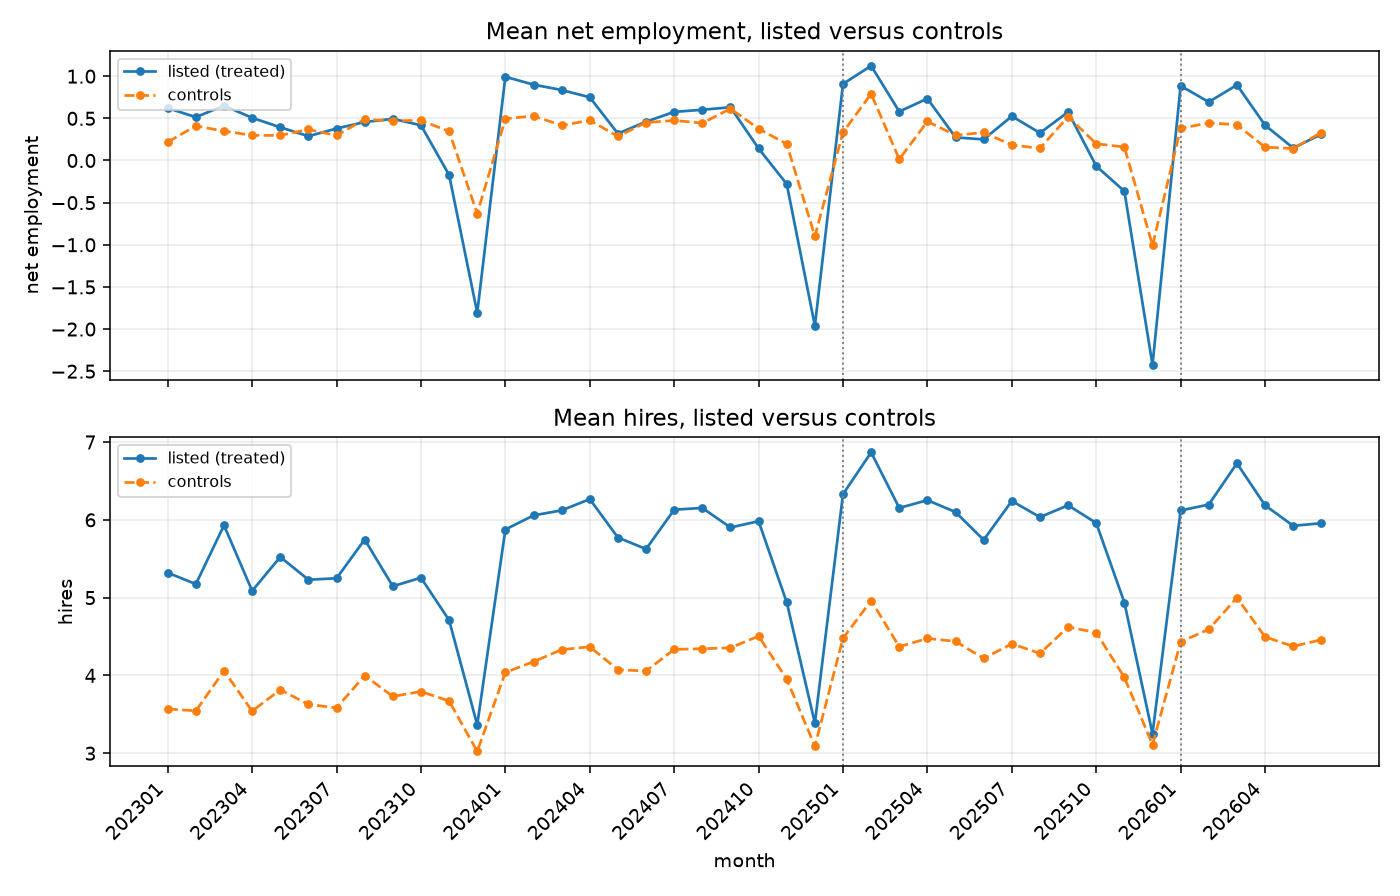
\includegraphics[width=0.95\textwidth]{fig_raw_means_listed_vs_controls.png}
\caption{Raw monthly means, listed classes and controls. Top: net employment. Bottom: hires. Descriptive only. Vertical lines mark January 2025 and January 2026.}
\label{fig:raw_means}
\end{figure}

\section{Method}
\label{sec:metodo}

The unit is class $s$, municipality $m$ and month $t$. $D_s=1$ if the class is on the list in articles 7 and 8 of Law 12.546, and 0 otherwise. $D_s$ is a time-invariant listing indicator.

\subsection{Why these fixed effects}

Listed and never-listed classes need not share the same calendar. A regression with only class, municipality and month fixed effects would leave that seasonality in the error, and would bias the year effects if the two groups load differently on the calendar. The principal specification therefore includes class×calendar month, municipality×civil month, class×municipality×calendar month and municipality×year. The contrast is across years within a calendar month and within a municipality. These fixed effects would be a bad control only if the policy worked by changing the seasonality of a class in a municipality. The leaner set, class$\times$calendar month plus municipality plus civil month, is kept as a comparison.
\subsection{Saturating the dose: $\beta_5$ and $\beta_{10}$}

Where the statutory dose takes values in $0,5$ or $10$ and every firm in a listed class receives the same ramp, it is possible to saturate the dose with a set of year dummies following \cite{callaway2024}: \begin{equation}
Y_{smt}=\delta_{s,c(t)}+\mu_{mt}+\alpha_{sm,c(t)}+\gamma_{m,\mathrm{year}(t)}+\beta_5 D_s\mathbf{1}(t\in 2025)+\beta_{10} D_s\mathbf{1}(t\in 2026)+\varepsilon_{smt}.
\label{eq:cgs_beta5_10_pt}
\end{equation} Here $c(t)\in\{1,\dots,12\}$ is the calendar month of $t$, and $\mu_{mt}$ is a municipality-by-year-month effect, the civil month. $t^*$ is January 2025, used in (2) and (3). The statutory dose, $\mathrm{Dose}_{st}$, is $5$ times $D_s$ in 2025 and $10$ times $D_s$ in 2026. The base period is 2023--24, and the 2026 term covers January through June. In this specification, $\beta_{5}$ captures the effect of the intervention for classes that are listed in 2025 compared to the base period. Similarly, $\beta_{10}$ captures the effect for classes listed in 2026 compared to the base period, not the differential effect between the two doses. Standard errors are clustered at the level of 4 digit class ($385$ classes, of which $137$ are listed).

A linear specification in $\text{Dose}_{st}\in\{0,5,10\}$ is included for comparison, but is not the preferred specification since it imposes a linear functional form on the dose response. It also pools 2025 and 2026 into a single per-point slope, which the saturation does not.
\subsection{The contrast $(\beta_{10}-\beta_5)/5$}

Table~\ref{tab:att_contrastes} also reports $\Delta=\hat\beta_{10}-\hat\beta_5$ and $\hat\Delta/5$, with standard errors clustered at the four-digit class level. Under parallel trends in $Y(0)$, $\beta_5$ and $\beta_{10}$ have the standard interpretation as the sectoral level effects of listing in 2025 and 2026.

Moreover, under strong parallel trends in dose (Theorem 3.3(d) in \citet{callaway2024}), $(\beta_{10}-\beta_5)/5$ is the average causal response to the step from $5$ to $10$ in dose. Without strong parallel trends in dose, the causal interpretation of this contrast can be affected by selection (Theorem 3.2 in \citet{callaway2024}). In this application the statute assigns dose 5 and dose 10 to the same listed classes, so the contrast does not compare two groups of units that received different doses; it compares the same group in two different years. This removes selection into dose, but it does not make strong parallel trends innocuous: $\beta_{10}-\beta_5$ also reflects (i) dynamic effects, since in 2026 the classes had already been exposed to dose 5 for a year; (ii) shocks specific to the listed classes between 2025 and 2026; and (iii) possible anticipation of the increases to 15\% and 20\%. We therefore read $(\beta_{10}-\beta_5)/5$ as the average causal response to the step from 5 to 10 only if these forces are negligible. The 2023 leads (Section 5.2) are a plausibility check on parallel trends in $Y(0)$; they are shared by the usual and the strong hypothesis.
\subsection{Event study: assigned dose, with a binary study alongside}

Event time is interacted with the assigned dose $W_{sk}$ : (i) zero if control; (ii) five if listed in 2023 and in 2025; (iii) ten if listed in year 2026. Because the class by municipality by calendar month effects are included, omitting all of calendar year 2024 from the event study is necessary, as just omitting a single month in 2024 would be the incorrect normalization. The coefficient $\theta_k$ at event time $k$ represents the approximate effect in that month per point. Then, the approximate level in years 2025 and 2026 is $5 \theta_{k}$ and $10 \theta_{k}$ respectively. Finally, in the pre period, the dose is set to five for leads so that the interactions in the pre period are not all zero.

Note that setting the dose to be the calendar dose, which would be zero for everyone in calendar years 2023 - 24 , and interacting that dose with event time would zero out all of the leads in an event study. Using the assigned dose prevents this. It is still possible to examine an event study for the binary variable for whether a class is listed in year $k$ to examine the timing of when they are affected. Moreover, to test parallel trends on $Y(0)$, one can examine the studentized maximum $T_{\max }$ for the twelve coefficients in calendar year 2023 of the event study for the binary variable of whether a class is listed in calendar year $k$, as is standard \citep{montiel2019,roth2023}. This test is also implied by $\theta_{k}=0$ in calendar year 2023 in the event study with assigned dose. This test does not reject for net employment in the principal sample (Section 6.5 reports the cuts).

Figure 3 re-estimates the same model omitting 2023 instead of 2024. With class-by-municipality-by-calendar-month and only two pre-years, this only reparametrizes the 2023 versus 2024 contrast: the 2024 coefficients in Figure 3 are the 2023 leads of Figure 2 with the sign reversed, and the timing placebo in Table~\ref{tab:placebo2024} is the same contrast again. These checks therefore cannot tell a pre-existing trend from anticipation in 2024, a year of high policy uncertainty (MP 1.202 in December 2023, partly revoked by MP 1.208 in February 2024, the STF injunction in ADI 7633, and the statute only in September). Extending the pre-period would be needed to separate them.



\section{Results}
\label{sec:results}
% =====================================================================

All of these employ a DiD design with a continuous treatment as in \citet{callaway2024}. The focus is on net employment; we also report hires, separations and starting wages from the same specification. All reported cells include p-values.

\subsection{Year effects for net employment}

As in \citet{callaway2024}, we will generally saturate the dose by including two dummies for the dose rather than a single slope on the calendar dose. Recall that the statutory dose only takes on 3 values (0, 5, and 10), and that they all follow the same ramp for each listed class. The main specification that we will use is given by equation \eqref{eq:cgs_beta5_10_pt}. These specifications include class$\times$calendar month, municipality$\times$civil month, class$\times$municipality$\times$calendar month and municipality$\times$year fixed effects. Standard errors are clustered at the 4-digit class level.

Table~\ref{tab:att_contrastes} reports $\beta_5$, $\beta_{10}$, $\Delta=\beta_{10}-\beta_5$ and $\Delta/5$ for four outcomes. In the first row, the outcome is net employment ($N=9{,}219{,}210$). Table~\ref{tab:att_contrastes} reports $\beta_5\simeq 0.020$, $\beta_{10}\simeq 0.011$, $\Delta\simeq -0.0087$ and $\Delta/5\simeq -0.0017$, with standard errors $0.043$, $0.062$, $0.065$ and $0.013$, and $p$-values $0.64$, $0.86$, $0.89$ and $0.89$. Thus, neither year effect in the principal specification is significantly different from zero. Hires and separations are also not statistically significant. For the logarithm of starting wages, results are similar, although the point estimates are even closer to zero; see Section~\ref{sec:wage_caveat}.

Table~\ref{tab:reta} reports the pooled slope on calendar dose under the principal specification, $0.0019$, with standard error $0.0056$ and $p$-value $0.74$, only for comparison.

How can we interpret $(\beta_{10}-\beta_5)/5$? Theorem 3.3(d) of \citet{callaway2024} shows that it equals the average causal response of a one point step change in dose from five to ten, if we assume strong parallel trends in dose. If we do not make that assumption, then $(\beta_{10}-\beta_5)/5$ reflects a combination of the effect of an incremental change in dose and selection, by Theorem 3.2. In this setting the statute assigns both doses to the same classes, so there is no selection into dose, but the contrast is exposed to the dynamic and group-specific forces discussed in Section 4.3. Under strong parallel trends in dose, and if those forces are negligible, we interpret $\hat\Delta/5$ as the average causal response to a one-point step change in dose from 5 to 10 for net employment. The 2023 leads are a plausibility check on parallel trends in $Y(0)$ (Section 5.2); they cannot distinguish the usual from the strong hypothesis, because in 2023 the assigned dose is five times the listing indicator, so the dose-$W$ and binary event studies coincide up to scale. The studentized maximum does not reject for any outcome (Table~\ref{tab:tmax}); the joint Wald test rejects for separations. Hires and separations are in any case too imprecise for the contrast to be informative, so we do not interpret $\hat\Delta/5$ for them.

\begin{table}[H]
\centering
\caption{Year effects and contrasts under the principal specification (principal).
$\beta_5$ and $\beta_{10}$ are the level effects of listing in 2025 and 2026 under parallel trends in Y(0).
$(\beta_{10}-\beta_5)/5$ is the average causal response of the step from dose 5 to dose 10 under the strong hypothesis, and if dynamic effects are negligible for net employment.
Cluster: four-digit class.
Each cell reports coef / s.e.\ / $p$.}
\label{tab:att_contrastes}
{\footnotesize
\setlength{\tabcolsep}{2.8pt}
\begin{tabular}{lcccccccccccc}
\toprule
Outcome & $\hat\beta_5$ & s.e. & $p$ & $\hat\beta_{10}$ & s.e. & $p$ & $\widehat{\Delta}$ & s.e. & $p$ & $\widehat{\Delta}/5$ & s.e. & $p$ \\
\midrule
\textbf{Net emp.} & $\mathbf{0.020}$ & $\mathbf{0.043}$ & $\mathbf{0.64}$ & $\mathbf{0.011}$ & $\mathbf{0.062}$ & $\mathbf{0.86}$ & $\mathbf{-0.0087}$ & $\mathbf{0.065}$ & $\mathbf{0.89}$ & $\mathbf{-0.0017}$ & $\mathbf{0.013}$ & $\mathbf{0.89}$ \\
Hires & $0.001$ & $0.147$ & $0.99$ & $-0.112$ & $0.243$ & $0.65$ & $-0.113$ & $0.120$ & $0.35$ & $-0.023$ & $0.024$ & $0.35$ \\
Separations & $-0.019$ & $0.171$ & $0.91$ & $-0.123$ & $0.240$ & $0.61$ & $-0.104$ & $0.087$ & $0.23$ & $-0.021$ & $0.017$ & $0.23$ \\
Log wage & $-0.0010$ & $0.0018$ & $0.58$ & $-0.0017$ & $0.0027$ & $0.54$ & $-0.0006$ & $0.0017$ & $0.71$ & $-0.0001$ & $0.0003$ & $0.71$ \\
\bottomrule
\end{tabular}}\\[0.4em]
{\footnotesize Notes: Flows $N=9{,}219{,}210$. Wage $N=2{,}222{,}824$ (0.3--150 times the minimum wage; cells with at most two hires and a mean contractual wage above BRL 50{,}000 dropped; August--September 2023 dropped, wages only).}
\end{table}

\subsection{Event study for net employment (assigned dose)}

The event study uses the same fixed effects as the year effects. Event time is interacted with the assigned dose $W_{sk}:$ 0 for a control class, 5 for a listed class in 2023 and in 2025, and 10 for a listed class in 2026. All of calendar year 2024 is omitted. In the pre-period $W_{sk}$ is kept at 5, as a lead scale, so that the pre-period interactions are not all zero.
\begin{equation}
Y_{smt}=\delta_{s,c(t)}+\mu_{mt}+\alpha_{sm,c(t)}+\gamma_{m,\mathrm{year}(t)}+\sum_{k\notin 2024}\theta_k W_{sk}\mathbf{1}\{t=t^{*}+k\}+\varepsilon_{smt}.
\end{equation}

\begin{figure}[H]
\centering
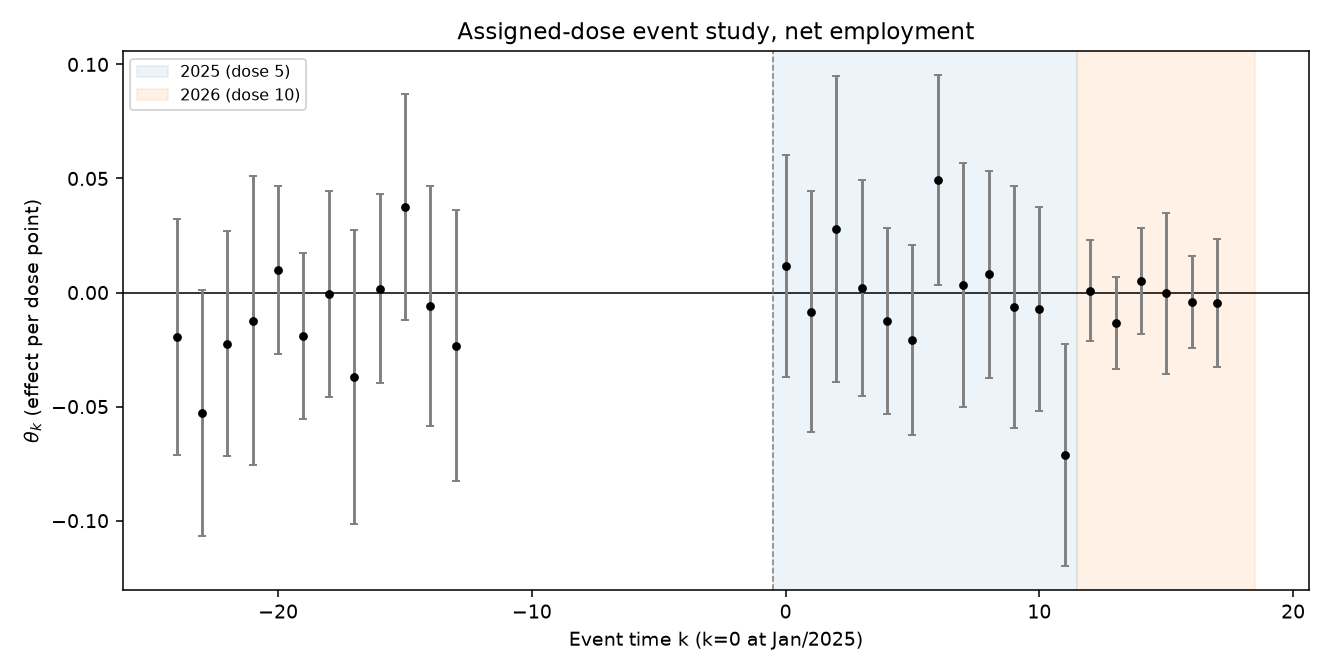
\includegraphics[width=0.95\textwidth]{fig_es_dose_base2024_saldo.png}
\caption{Assigned-dose event study for net employment. Base year 2024 omitted. Pre-period $W=5$ is a lead scale.}
\label{fig:es_dose_saldo}
\end{figure}
The coefficient $\theta_k$ is a per-point effect in that month: $5\theta_k$ is the 2025 level and $10\theta_k$ is the 2026 level. Figure~\ref{fig:es_dose_saldo} shows net employment. Most coefficients are small and their intervals include zero, but the path is not uniformly flat: the 2023 leads are mostly negative, and the intervals for July 2025 ($k=6$) and December 2025 ($k=11$) exclude zero in Figures 2 and 4 (one or two such cases among 30 coefficients would not be unusual). The studentized maximum on the twelve 2023 coefficients does not reject for net employment (Table~\ref{tab:tmax}, $p\approx0.43$); the joint Wald statistic is 13.30 ($\text{df}=12$, $p\approx0.35$). These leads compare 2023 with the 2024 base only, so they have limited power.

\begin{figure}[H]
\centering
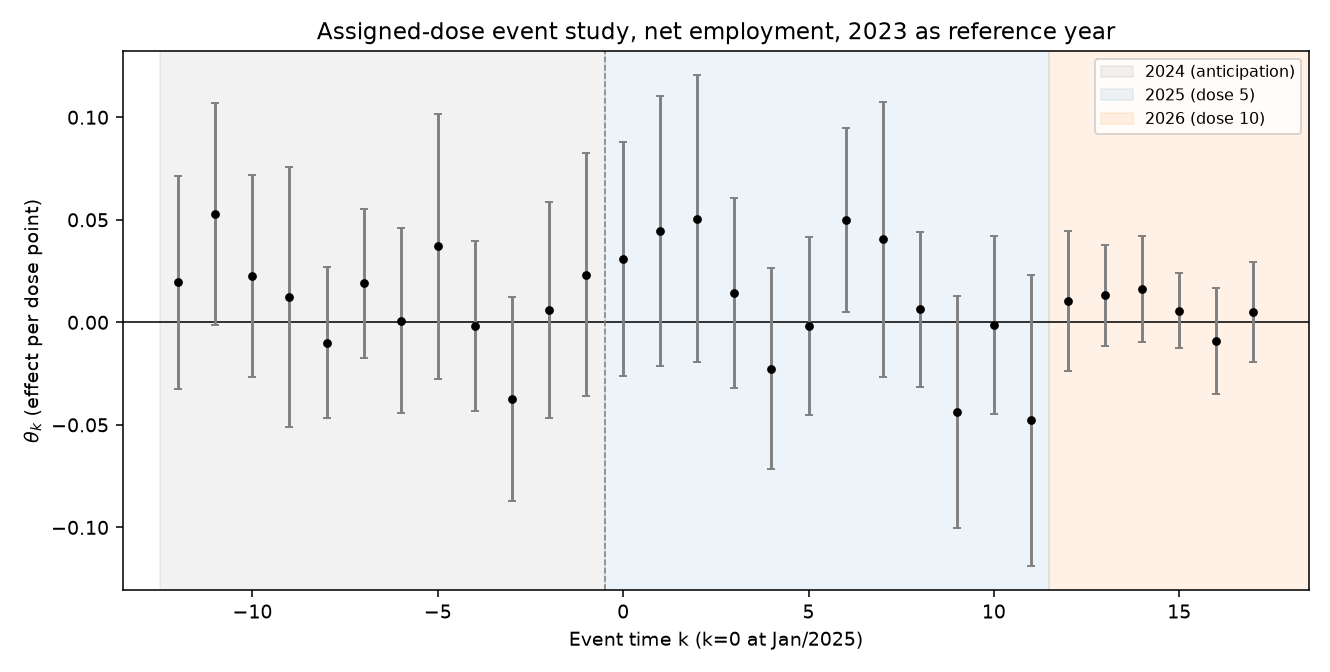
\includegraphics[width=0.92\textwidth]{fig_es_dose_base2023_saldo.png}
\caption{Assigned-dose event study for net employment, 2023 omitted and 2024 left free. The gray band is the anticipation window. Same contrast as the 2023 leads of Figure 2, with the sign reversed.}
\label{fig:es_base2023}
\end{figure}

\subsection{Binary event study and usual parallel trends}

A binary listed$\times$event-time study sits alongside as exposure timing, not as the preferred plot (Figure~\ref{fig:es_bin_saldo}). It uses the same fixed effects. The regressor is the listing indicator $D_s$, equal to 1 if the class is on the list.
\begin{equation}
\begin{aligned}
Y_{smt}
&=
\delta_{s,c(t)}+\mu_{mt}+\alpha_{sm,c(t)}+\gamma_{m,\mathrm{year}(t)} \\
&\quad
+\sum_{k\notin 2024}\theta_k\, D_s\,\mathbf{1}\{t=t^{*}+k\}
+\varepsilon_{smt}.
\end{aligned}
\label{eq:es_bin}
\end{equation}
\begin{figure}[H]
\centering
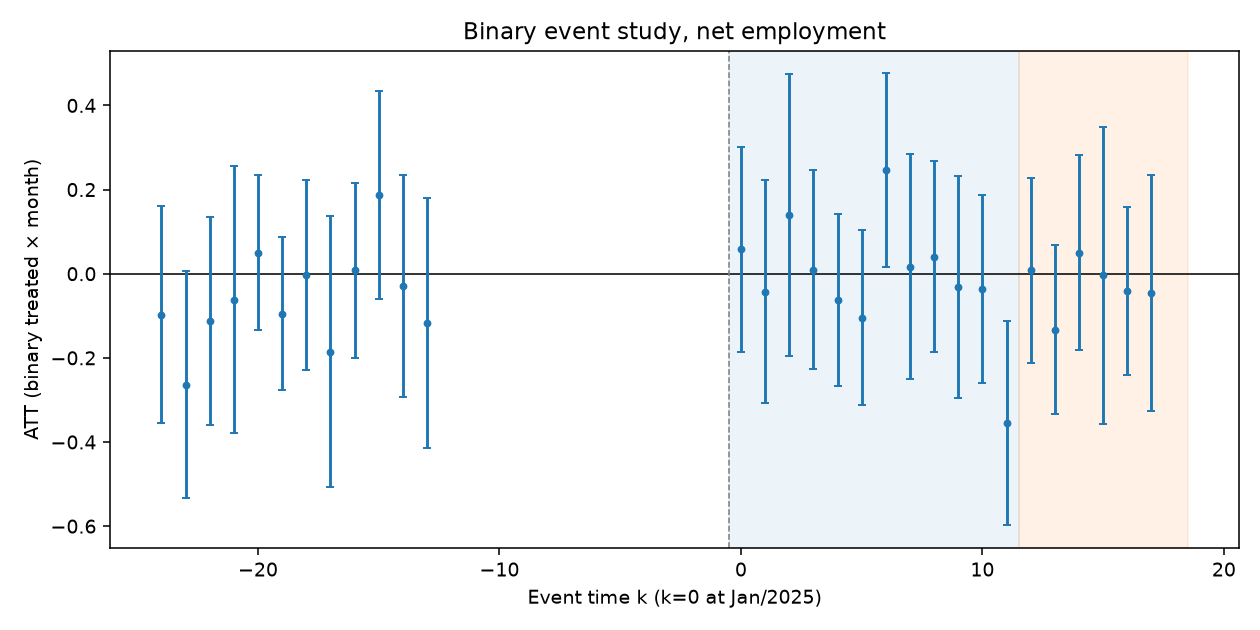
\includegraphics[width=0.95\textwidth]{fig_es_binario_base2024_saldo.png}
\caption{Binary event study for net employment: listed times event time. Exposure timing. Base year 2024 omitted.}
\label{fig:es_bin_saldo}
\end{figure}

Binary event studies for hires, separations and starting wages are in Appendix B.

\subsection{Supporting outcomes}
\label{sec:apoio}

Table~\ref{tab:att_contrastes} also reports hires and separations from the same specification. Their standard errors, 0.15 to 0.24, are small relative to the means of 5.65 and 5.35 hires and separations per cell-month, but the intervals still accommodate effects of a few percent of the flow, large enough to be compatible with the net-employment result. These columns are uninformative about effects of that size. The 2026 point estimates for hires ($-0.112$) and separations ($-0.123$) have the same sign and similar size, which would be consistent with lower turnover and no change in net employment, but neither is distinguishable from zero ($p=0.65$ and $0.61$). We do not interpret them as evidence of reduced turnover. A direct test would use turnover (hires plus separations) as the outcome. The assigned-dose event studies are in Appendix A.

\subsection{Starting Wages}\label{sec:wage_caveat}

Regarding the impact on the log of starting wages, although we also observe an almost null impact (year effect $p$-values of around $0.58$ and $0.54$), we believe that these results are less robust to the specification choices that we make (namely, the joint Wald test on the 2023 leads yields $p\approx0.053$, although the studentized maximum does not reject; Table~\ref{tab:tmax}). For the sake of completeness, we include the wage results in Table~\ref{tab:att_contrastes}. However, we would like to stress that we do not consider the wage results as supportive of the null hypothesis in the net-employment column. We also only show the dose-$W$ figure for wages in the appendix.
% =====================================================================
\section{Robustness}
\label{sec:robustness}
% =====================================================================

\subsection{Timing placebo under ordinary parallel trends}

Truncating the sample so that the "treatment" occurred in 2024, none of the coefficients is statistically significant in the main specification. The effect on net employment is 0.060 (se = 0.051, p-value = 0.24) with $5{,}268{,}120$ observations. Supporting outcomes have coefficients of 0.066 (se = 0.176, p-value = 0.71) for hires, 0.006 (se = 0.170, p-value = 0.97) for separations, and -0.0016 (se = 0.0018, p-value = 0.37, N = $886{,}846$) for log starting wage. This is the same 2023 versus 2024 contrast as the leads in Figure 2 and the 2024 coefficients in Figure 3 (Section 4.4). Its size (0.060, three times $\hat\beta_5$) is a natural benchmark for how much a pre-existing drift could matter.

\begin{table}[H]
\centering
\caption{Timing placebo: false treatment year 2024, sample through December 2024, principal specification.}
\label{tab:placebo2024}
\begin{tabular}{lrrrr}
\toprule
Outcome & coef. & s.e. & $p$ & $N$ \\
\midrule
\textbf{Net Employment} & $\mathbf{0.060}$ & $\mathbf{0.051}$ & $\mathbf{0.24}$ & 5{,}268{,}120 \\
Hires & 0.066 & 0.176 & 0.71 & 5{,}268{,}120 \\
Separations & 0.006 & 0.170 & 0.97 & 5{,}268{,}120 \\
Log starting wage & $-0.0016$ & 0.0018 & 0.37 & 886{,}846 \\
\bottomrule
\end{tabular}
\end{table}

\subsection{Joint pre-test on the assigned-dose event study}

Table~\ref{tab:tmax} reports, for each outcome, the studentized maximum on the 2023 leads of the binary event study, which is our criterion, next to the joint Wald test on the 2023 leads of the assigned-dose event study. Because the assigned dose is five times the listing indicator in 2023, the two event studies are the same up to scale and test the same restriction. The Wald test is more sensitive to correlated deviations: it rejects for separations ($p\approx0.020$) and is borderline for log starting wages ($p\approx0.053$), while the studentized maximum rejects for none in the principal specification.

\begin{table}[H]
\centering
\caption{Joint tests on the 2023 leads (base year 2024), principal specification. $T_{\max}$: studentized maximum on the binary event study (our criterion). Wald: joint test of $\theta_k=0$ on the assigned-dose event study; in 2023 the two event studies coincide up to scale.}
\label{tab:tmax}
\begin{tabular}{lccccccc}
\toprule
Outcome & $T_{\max}$ & Crit.\ 5\% & $p_{\max}$ & Wald & df & $p_{\text{Wald}}$ & Leads \\
\midrule
Net employment & 1.92 & 2.82 & 0.43 & 13.30 & 12 & 0.347 & 12 \\
Hires & 1.12 & 2.56 & 0.71 & 14.43 & 12 & 0.274 & 12 \\
Separations & 1.48 & 2.57 & 0.42 & 24.08 & 12 & 0.020 & 12 \\
Log starting wage & 1.93 & 2.78 & 0.41 & 18.09 & 10 & 0.053 & 10 \\
\bottomrule
\end{tabular}
\end{table}

\subsection{Leaner specification, as a comparison only}

Table~\ref{tab:lean} displays the same year average treatment effects, but now estimated through a leaner specification \footnote{The lean specification simply uses \texttt{class $\times$ calendar month, municipality, and civil month} as the set of variables defining the groups.}. The exercise aims to verify whether the lack of rejection of the null of the former specification was due to an oversaturation of the groups. It does not. Notice that the coefficients are essentially the same as in the principal specification.

\begin{table}[H]
\centering
\caption{Year effects under leaner specification (comparison only).}
\label{tab:lean}
{\footnotesize
\setlength{\tabcolsep}{3pt}
\begin{tabular}{lcccccccc}
\toprule
Outcome & $\hat\beta_5$ & s.e. & $p$ & $\hat\beta_{10}$ & s.e. & $p$ & $\widehat{\Delta}/5$ & $p$ \\
\midrule
Net employment & $0.023$ & $0.039$ & $0.55$ & $0.016$ & $0.058$ & $0.79$ & $-0.0015$ & $0.91$ \\
Hires & $-0.001$ & $0.132$ & $0.99$ & $-0.112$ & $0.226$ & $0.62$ & $-0.022$ & $0.34$ \\
Separations & $-0.024$ & $0.150$ & $0.87$ & $-0.127$ & $0.216$ & $0.55$ & $-0.021$ & $0.21$ \\
Log wage & $-0.0009$ & $0.0017$ & $0.60$ & $-0.0023$ & $0.0025$ & $0.36$ & $-0.0003$ & $0.36$ \\
\bottomrule
\end{tabular}}
\end{table}

\subsection{Line on the dose, as a comparison only}

Table~\ref{tab:reta} reports the pooled slope on calendar dose under the principal specification.
For net employment the coefficient is $0.0019$ (s.e.\ $0.0056$, $p\approx 0.74$). The line imposes linearity across $\{0,5,10\}$ and is retained only as a comparison column.

\begin{table}[H]
\centering
\caption{Pooled linear dose under the principal specification (comparison column only).
Cluster: four-digit class}
\label{tab:reta}
\begin{tabular}{lccc}
\toprule
Outcome & coef & s.e. & $p$ \\
\midrule
Net employment & 0.0019 & 0.0056 & 0.738 \\
Hires  & $-0.0081$ & 0.0253 & 0.748 \\
Separations  & $-0.0100$ & 0.0265 & 0.706 \\
Log starting wage & $-0.00018$ & 0.00028 & 0.536 \\
\bottomrule
\end{tabular}
\end{table}

\subsection{Sample cuts (drop construction; divisions with a listed class)}
\label{sec:rob_samples}

This table re-estimates the principal year effects and event studies on the restricted samples. The specification is always the principal one, with FE parameterized as $\delta_{s,c(t)} + \mu_{mt} + \alpha_{sm,c(t)} + \gamma_{m, \text{year}(t)}$ 

\begin{enumerate}[nosep]
  \item \textbf{Principal (full sample).} Full sample : $N=9{,}219{,}210$ flow cells.
  \item \textbf{Drop section F (construction).} Drop cells with CNAE section~$=$~F. $N=7{,}754{,}460$.
  \item \textbf{CNAE-2 divisions with at least one listed class.} Restrict controls to two-digit divisions that contain $\geq 1$ listed class ($n_{\mathrm{divs}}=27$). $N=6{,}294{,}582$.
\end{enumerate}

Table~\ref{tab:att_rob} presents the same year effects on the discrete dose $\{0,5,10\}$. For net employment, the year effects remain insignificant in both cuts: without construction, $\beta_5=0.084$ (s.e.\ $=0.055$, $p=0.13$), $\beta_{10}=0.026$ (s.e.\ $=0.070$, $p=0.71$) and $\Delta/5=-0.011$ (s.e.\ $=0.016$, $p=0.47$); in the CNAE-2 cut, $\beta_5=0.012$ (s.e.\ $=0.044$, $p=0.79$), $\beta_{10}=0.071$ (s.e.\ $=0.069$, $p=0.30$) and $\Delta/5=0.012$ (s.e.\ $=0.012$, $p=0.32$). The pre-trend check does not travel with them. Without construction, the studentized maximum on the 2023 leads of net employment rejects ($T_{\max}=3.40$, 5\% critical value $2.81$, $p=0.0068$). Separations in that cut do not ($p=0.095$). In the CNAE-2 cut, no outcome rejects; for net employment, $T_{\max}=2.47$ ($p=0.13$).

\begin{table}[H]
\centering
\caption{Year effects under the principal specification across samples (principal; drop section~F; CNAE-2 with listed).
Cluster: four-digit class. Each cell: coef / s.e.\ / $p$.}
\label{tab:att_rob}
{\scriptsize
\setlength{\tabcolsep}{2.2pt}
\begin{tabular}{llccccccccc}
\toprule
Outcome & Sample & $\hat\beta_5$ & s.e. & $p$ & $\hat\beta_{10}$ & s.e. & $p$ & $\widehat{\Delta}/5$ & s.e. & $p$ \\
\midrule
\multirow{3}{*}{\textbf{Net emp.}}
 & Principal & $\mathbf{0.020}$ & $\mathbf{0.043}$ & $\mathbf{0.64}$ & $\mathbf{0.011}$ & $\mathbf{0.062}$ & $\mathbf{0.86}$ & $\mathbf{-0.0017}$ & $\mathbf{0.013}$ & $\mathbf{0.89}$ \\
 & no construction & $0.084$ & $0.055$ & $0.13$ & $0.026$ & $0.070$ & $0.71$ & $-0.011$ & $0.016$ & $0.47$ \\
 & CNAE-2 & $0.012$ & $0.044$ & $0.79$ & $0.071$ & $0.069$ & $0.30$ & $0.012$ & $0.012$ & $0.32$ \\
\midrule
\multirow{3}{*}{Hires}
 & Principal & $0.001$ & $0.147$ & $0.99$ & $-0.112$ & $0.243$ & $0.65$ & $-0.023$ & $0.024$ & $0.35$ \\
 & no construction & $-0.066$ & $0.186$ & $0.72$ & $-0.155$ & $0.339$ & $0.65$ & $-0.018$ & $0.034$ & $0.60$ \\
 & CNAE-2 & $0.079$ & $0.171$ & $0.64$ & $-0.001$ & $0.259$ & $1.00$ & $-0.016$ & $0.023$ & $0.49$ \\
\midrule
\multirow{3}{*}{Separations}
 & Principal & $-0.019$ & $0.171$ & $0.91$ & $-0.123$ & $0.240$ & $0.61$ & $-0.021$ & $0.017$ & $0.23$ \\
 & no construction & $-0.150$ & $0.221$ & $0.50$ & $-0.181$ & $0.328$ & $0.58$ & $-0.006$ & $0.024$ & $0.79$ \\
 & CNAE-2 & $0.068$ & $0.189$ & $0.72$ & $-0.071$ & $0.289$ & $0.81$ & $-0.028$ & $0.023$ & $0.22$ \\
\midrule
\multirow{3}{*}{Log wage}
 & Principal & $-0.0010$ & $0.0018$ & $0.58$ & $-0.0017$ & $0.0027$ & $0.54$ & $-0.0001$ & $0.0003$ & $0.71$ \\
 & no construction & $-0.0017$ & $0.0021$ & $0.43$ & $-0.0043$ & $0.0030$ & $0.16$ & $-0.0005$ & $0.0004$ & $0.16$ \\
 & CNAE-2 & $0.0000$ & $0.0023$ & $0.98$ & $0.0012$ & $0.0031$ & $0.70$ & $0.0002$ & $0.0004$ & $0.51$ \\
\bottomrule
\end{tabular}}\\[0.35em]
{\footnotesize Notes: $N$ (flows) = 9{,}219{,}210 (principal); 7{,}754{,}460 (no construction); 6{,}294{,}582 (CNAE-2).
Wage $N$ = 2{,}222{,}824; 1{,}904{,}720; 1{,}545{,}212.}
\end{table}

\paragraph{Event studies on the cuts.}
Figures~ \ref{fig:es_dose_semF_saldo} --\ref{fig:es_dose_CNAE-2_saldo} report the preferred dose-$W$ paths of net employment for the preferred specification in each cut (Base 2024 is omitted. All use the same dose-$W$ coding as in the main text). Further dose-$W$ figures for hires, separations and starting wages in both cuts are in Appendix C.

\begin{figure}[H]
\centering
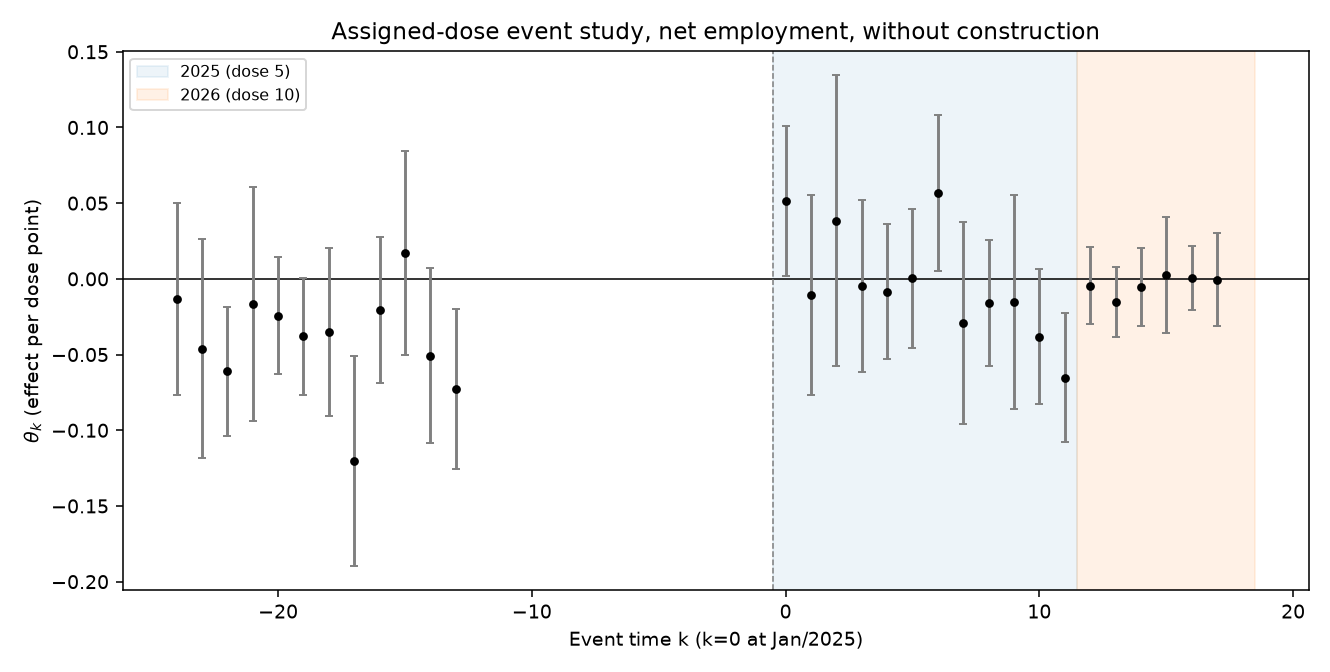
\includegraphics[width=0.95\textwidth]{fig_es_dose_semF_base2024_saldo.png}
\caption{Dose-$W$ event study for net employment, drop section~F (no construction), principal specification, base 2024 omitted.}
\label{fig:es_dose_semF_saldo}
\end{figure}

\begin{figure}[H]
\centering
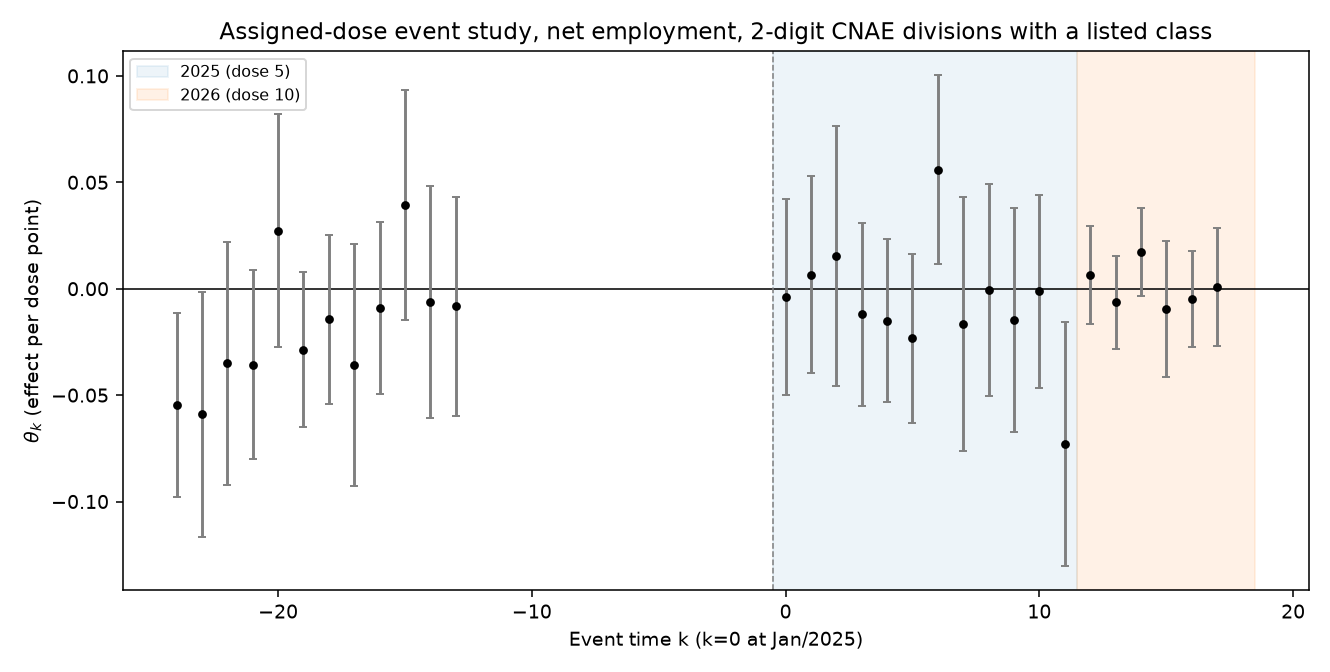
\includegraphics[width=0.95\textwidth]{fig_es_dose_cnae2_base2024_saldo.png}
\caption{Dose-$W$ event study for net employment, CNAE-2 divisions with listed class, principal specification, base 2024 omitted.}
\label{fig:es_dose_CNAE-2_saldo}
\end{figure}

\section{Discussion}
\label{sec:discussao}
% =====================================================================

Our estimates for net employment are small and statistically indistinguishable from zero in the short run (listed for 2025 and the first half of 2026), but they are imprecise, as discussed below. The underlying unit of analysis is the flow panel of completed CAGED records and our preferred specification includes class$\times$calendar month, municipality$\times$civil month, class$\times$municipality$\times$calendar month and municipality$\times$year fixed effects, with standard errors clustered by four-digit class. We employ two alternative sample cuts, none with statistically significant year effects (see Section \ref{sec:rob_samples}).

First, recall that firms selecting the hybrid path are legally constrained to maintain at least 75\% of last year's average employment. The rule limits a large fall in the average stock. Hires and separations that offset each other are not constrained, so a lower turnover can still show up in the flows. Second, the post-period is short: it ends in June 2026, giving only 18 months of phase-in before the statutory increases to 15\% in 2027 and 20\% in 2028. Third, the parameter is a sector-level intention to treat. A cell mixes establishments, and Simples Nacional establishments are outside the statute. That mix attenuates the contrast. It can explain a small estimate.

The listed classes are not a random sample. A shock specific to those sectors in 2025--26 would bias the contrast. That is a threat to validity. The 2023 leads, twelve months against the 2024 base, do not reject for net employment in the principal sample (studentized maximum $p\approx0.43$; joint Wald $p\approx0.35$), but the studentized maximum does reject when construction is dropped ($p=0.0068$; Section 6.5), so the absence of rejection in the full sample is not robust to the choice of sample.

The exercise fails to reject a zero effect for net employment, but it does not rule out a large one: the 95 percent interval for $\beta_5$ is about $[-0.064,\,0.104]$ and for $\beta_{10}$ about $[-0.11,\,0.13]$, against a mean net employment of 0.30 per cell-month. The intervals for hires and separations still accommodate effects of a few percent of the flow, so those columns are uninformative rather than supportive of a null. The contrast $(\beta_{10}-\beta_5)/5$ is also imprecise (point estimate $-0.0017$, 95\% interval about $[-0.027,\,0.024]$ per point). A high $p$-value does not mean that the true response is small.

The year effects for hires, separations and starting wages are not statistically significant either, but the first two are too imprecise to be informative; the assigned-dose paths are in Appendix A. For starting wages, the joint Wald test on the 2023 leads is borderline ($p\approx0.053$), although the studentized maximum does not reject ($p\approx0.41$).

As more months of CAGED become available, we will extend the post-period to further explore these effects. Extending the pre-period to 2021--22 would also allow us to separate pre-existing trends from anticipation in 2024.

% =====================================================================
\section{Conclusion}
\label{sec:conclusion}
% =====================================================================

This paper uses a DiD design with continuous treatment to study the short-run, intent-to-treat association between the re-taxation of some Brazilian payroll charges in 2025-26 (Law 14.973/2024) and formal job market flows as documented by the CAGED administrative dataset. The treatment "dose" takes only three values, $\{0, 5, 10\}$. The analysis takes net employment as its anchor outcome. The main specification saturates the dose with two year effects, $\beta_5$ for 2025 and $\beta_{10}$ for 2026, interpreted as intention-to-treat effects at the class level, relative to the base years 2023--24, with class$\times$calendar-month, municipality$\times$civil-month, class$\times$municipality$\times$calendar-month and municipality$\times$year fixed effects, and clusters the standard errors.

The main specification finds small point estimates, none statistically significant: $\hat\beta_5\approx 0.020$ (95\% CI $[-0.064,\,0.104]$) and $\hat\beta_{10}\approx 0.011$ (95\% CI $[-0.11,\,0.13]$), against a mean net employment of 0.30 per cell-month. The intervals do not rule out large effects. The contrast $\widehat{\Delta}/5\approx -0.0017$ is the average causal response to the step from 5 to 10 only under strong parallel trends, and if dynamic effects and shocks specific to the listed classes are negligible (Section 4.3). A test based on the studentized maximum statistic across all 2023 coefficients gives $T_{\max}\approx 1.92$ ($p\approx 0.43$), which does not reject usual parallel trends for net employment. The same test rejects for net employment when construction is dropped ($T_{\max}=3.40$, $p=0.0068$; Section 6.5). The joint Wald test on the same leads also fails to reject for net employment ($p\approx0.35$), but it rejects for separations ($p\approx0.020$) and is borderline for starting wages ($p\approx0.053$), whereas the studentized maximum rejects for none in the principal specification. We therefore interpret the contrast only for net employment; for hires and separations the estimates are too imprecise to be informative, and for starting wages the evidence on pre-trends is mixed. The comparison columns consider a "leaner" specification (class$\times$calendar month, municipality, and civil month) and the slope of the dose in a linear specification. Two sample cuts are considered, both with the main specification: (i) construction classes are dropped; (ii) the control group is restricted to divisions that contain at least one listed class. Both cuts give year effects on net employment that are not statistically significant, although $\hat\beta_5$ is larger without construction (0.084).

% =====================================================================
\appendix
\section{Supporting dose-$W$ event studies}
\label{app:es_apoio}
% =====================================================================

Figures~\ref{fig:es_dose_adm}--\ref{fig:es_dose_wage} report preferred dose-$W$ event studies for hires, separations, and log starting wages under the principal specification. Net employment is in Figure~\ref{fig:es_dose_saldo}.

\begin{figure}[H]
\centering
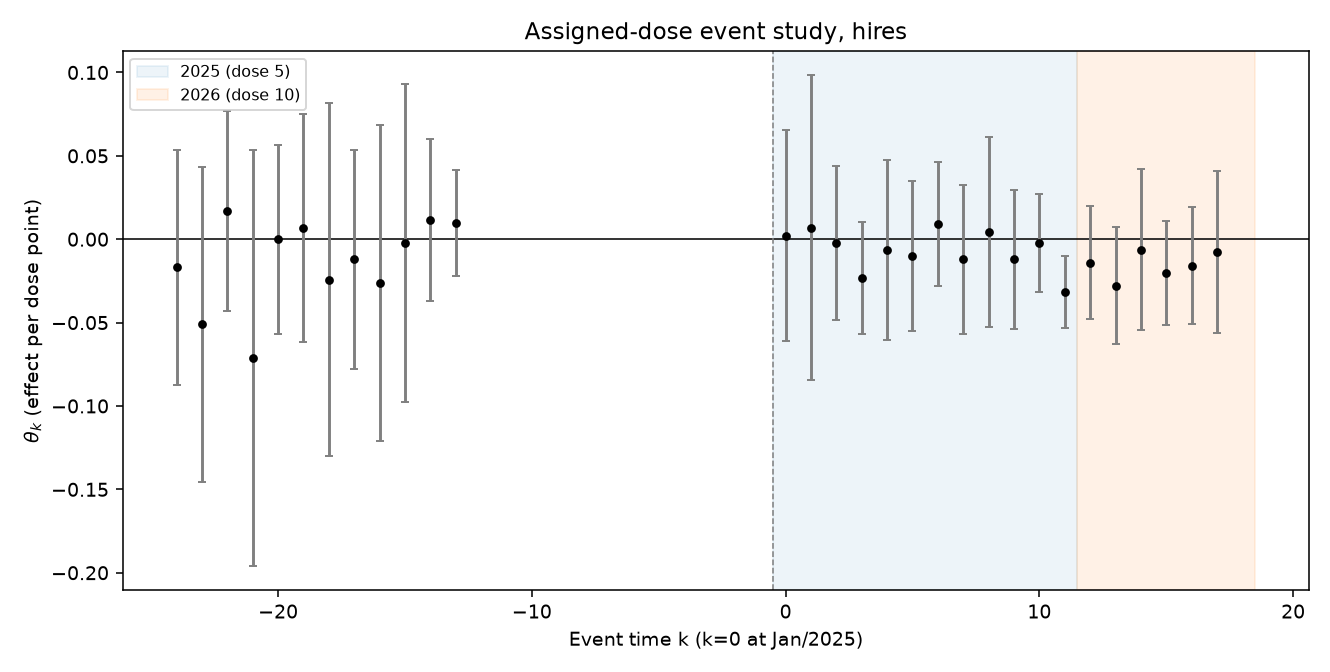
\includegraphics[width=0.95\textwidth]{fig_es_dose_base2024_admitidos.png}
\caption{Dose-$W$ event study for hires, principal specification. Base 2024 omitted; pre $W=5$ is lead scale.}
\label{fig:es_dose_adm}
\end{figure}

\begin{figure}[H]
\centering
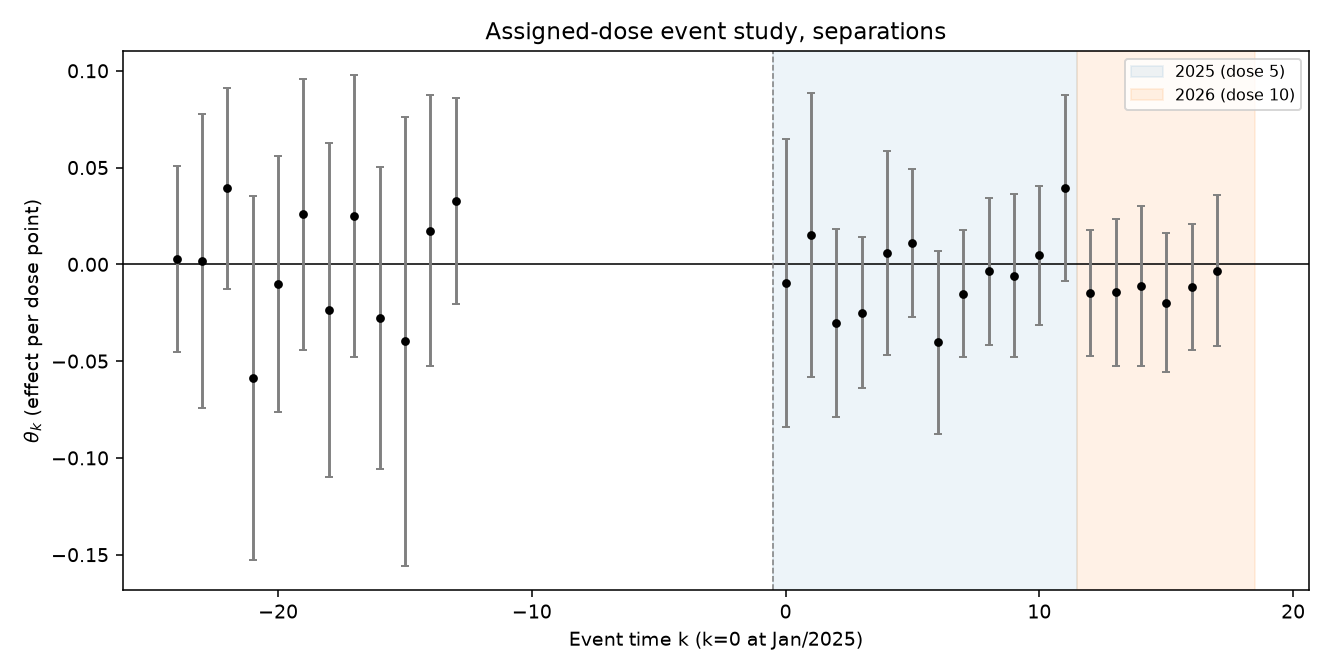
\includegraphics[width=0.95\textwidth]{fig_es_dose_base2024_desligados.png}
\caption{Dose-$W$ event study for separations, principal specification. Base 2024 omitted; pre $W=5$ is lead scale.
Joint Wald test on the 2023 leads: $p\approx0.020$ (studentized maximum: $p\approx0.42$).}
\label{fig:es_dose_des}
\end{figure}

\begin{figure}[H]
\centering
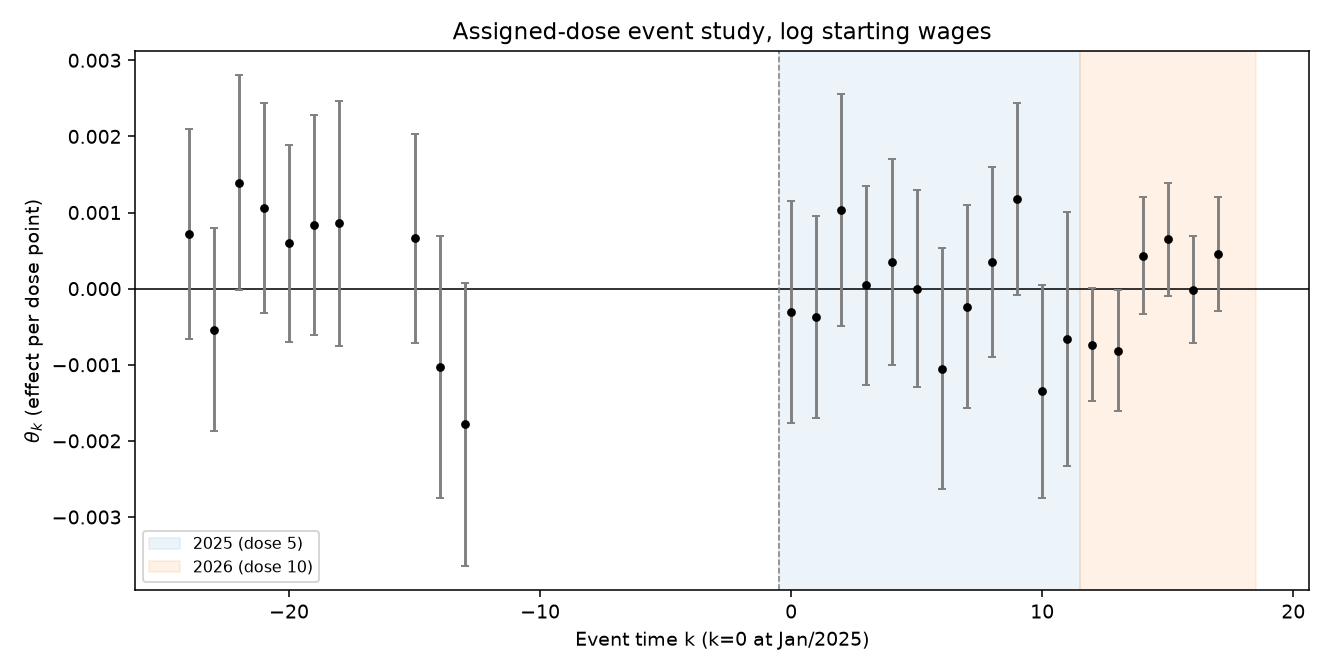
\includegraphics[width=0.95\textwidth]{fig_es_dose_base2024_log_salario.png}
\caption{Dose-$W$ event study for log starting wages, principal specification.
Joint Wald test on the 2023 leads: $p\approx0.053$ (studentized maximum: $p\approx0.41$).}
\label{fig:es_dose_wage}
\end{figure}

\subsection*{A.2 Same event studies with 2023 omitted}
Figures 10--12 repeat the assigned-dose event studies for hires, separations and log starting wages omitting 2023 and leaving 2024 free. They reparametrize Figures 7--9 (Section 4.4) and are not an independent check of anticipation; the joint tests on the 2024 coefficients are those of the 2023 leads in Table~\ref{tab:tmax}, with the sign reversed.

\begin{figure}[H]
\centering
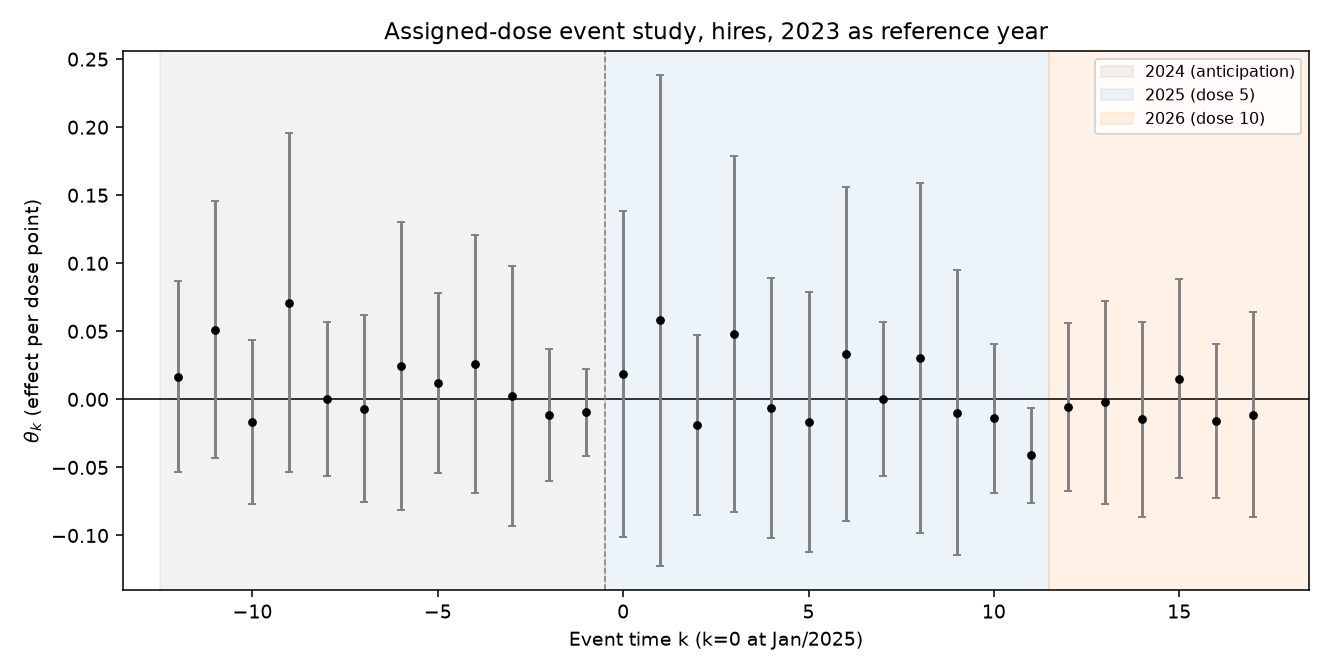
\includegraphics[width=0.92\textwidth]{fig_es_dose_base2023_admitidos.png}
\caption{Assigned-dose event study for hires, 2023 omitted and 2024 left free. Gray band: anticipation window.}
\label{fig:es_base2023_hires}
\end{figure}

\begin{figure}[H]
\centering
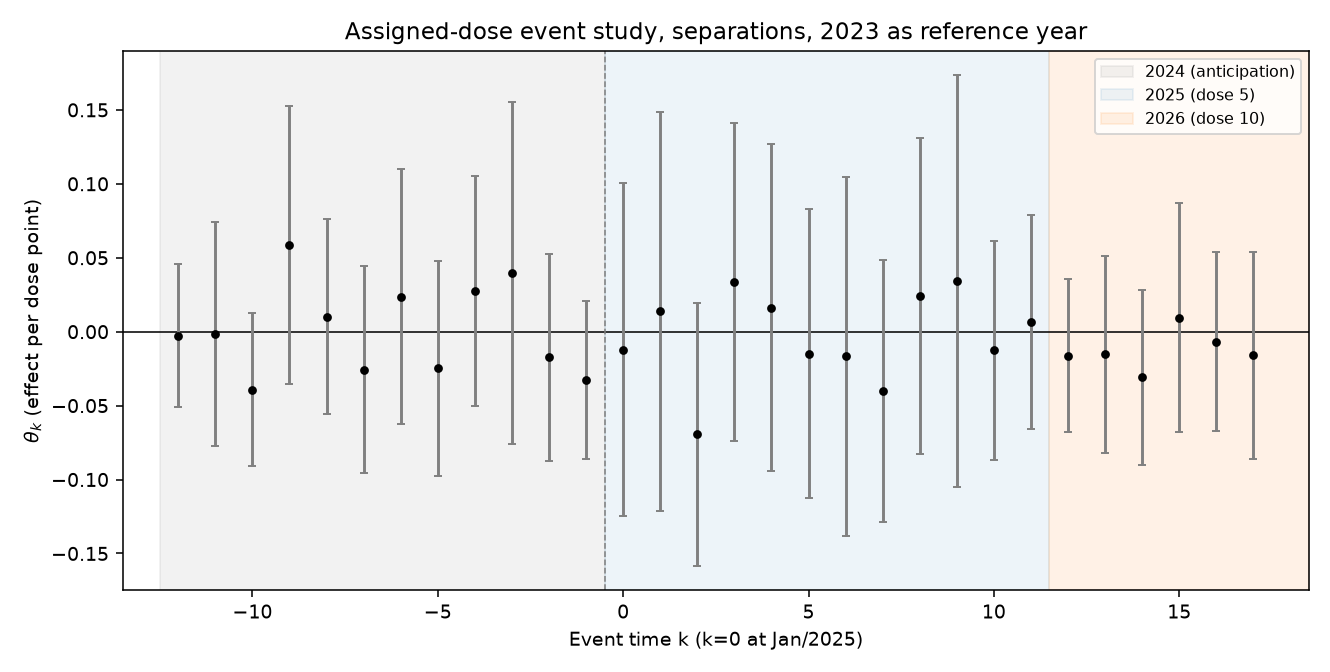
\includegraphics[width=0.92\textwidth]{fig_es_dose_base2023_desligados.png}
\caption{Assigned-dose event study for separations, 2023 omitted and 2024 left free. Gray band: anticipation window.}
\label{fig:es_base2023_sep}
\end{figure}

\begin{figure}[H]
\centering
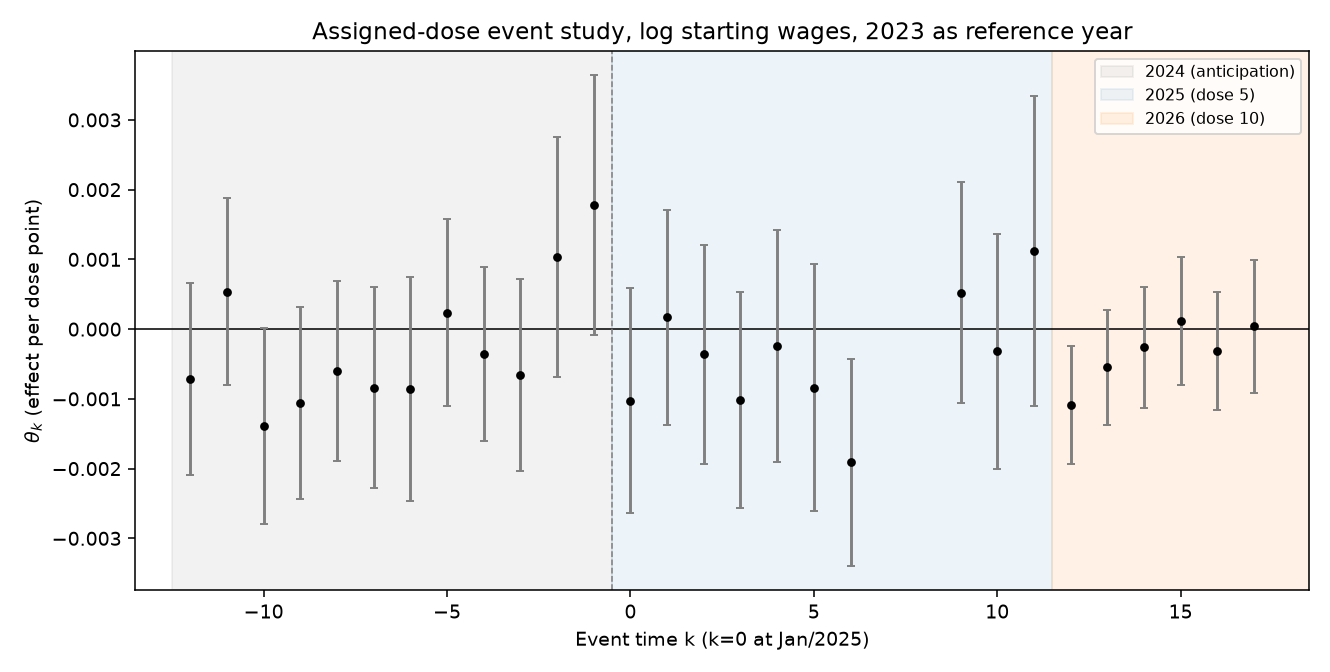
\includegraphics[width=0.92\textwidth]{fig_es_dose_base2023_log_salario.png}
\caption{Assigned-dose event study for log starting wages, 2023 omitted and 2024 left free. Gray band: anticipation window.
August and September 2023 are dropped from the wage sample, so with 2023 omitted the August and September 2025 coefficients ($k=7,8$) are not identified.}
\label{fig:es_base2023_wage}
\end{figure}

\section{Binary ES for supporting outcomes}
\label{app:es_bin}
% =====================================================================

\begin{figure}[H]
\centering
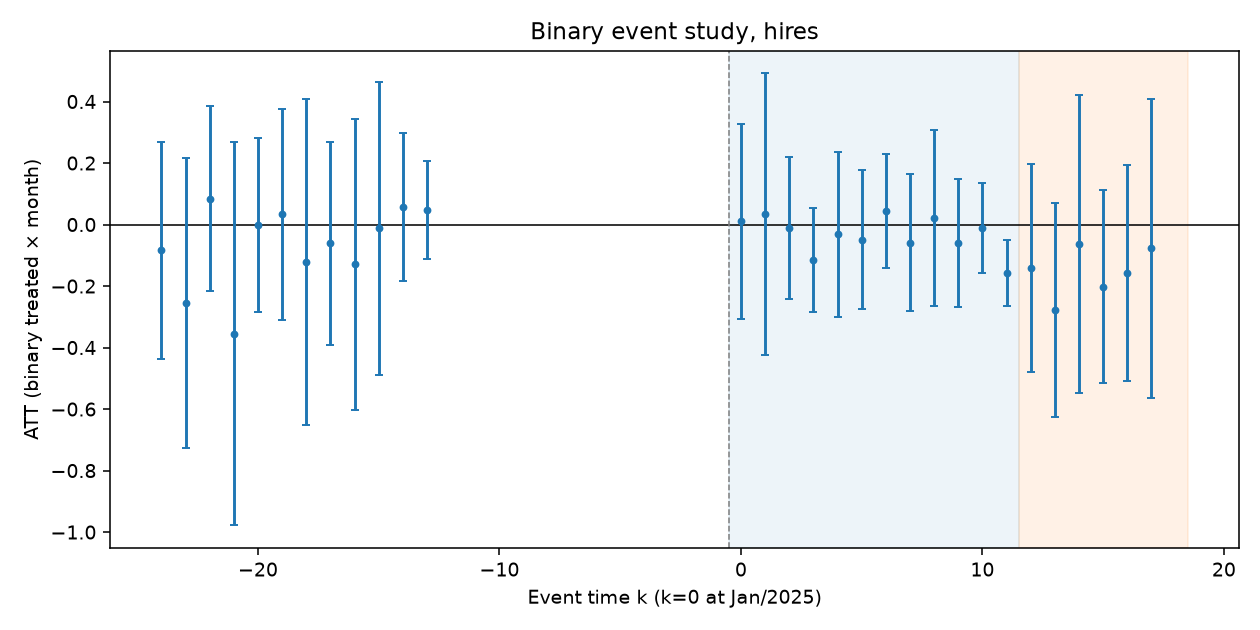
\includegraphics[width=0.95\textwidth]{fig_es_binario_base2024_admitidos.png}
\caption{Binary ES for hires (exposure timing), principal specification. $T_{\max}$ $p\approx 0.71$.}
\label{fig:es_bin_adm}
\end{figure}

\begin{figure}[H]
\centering
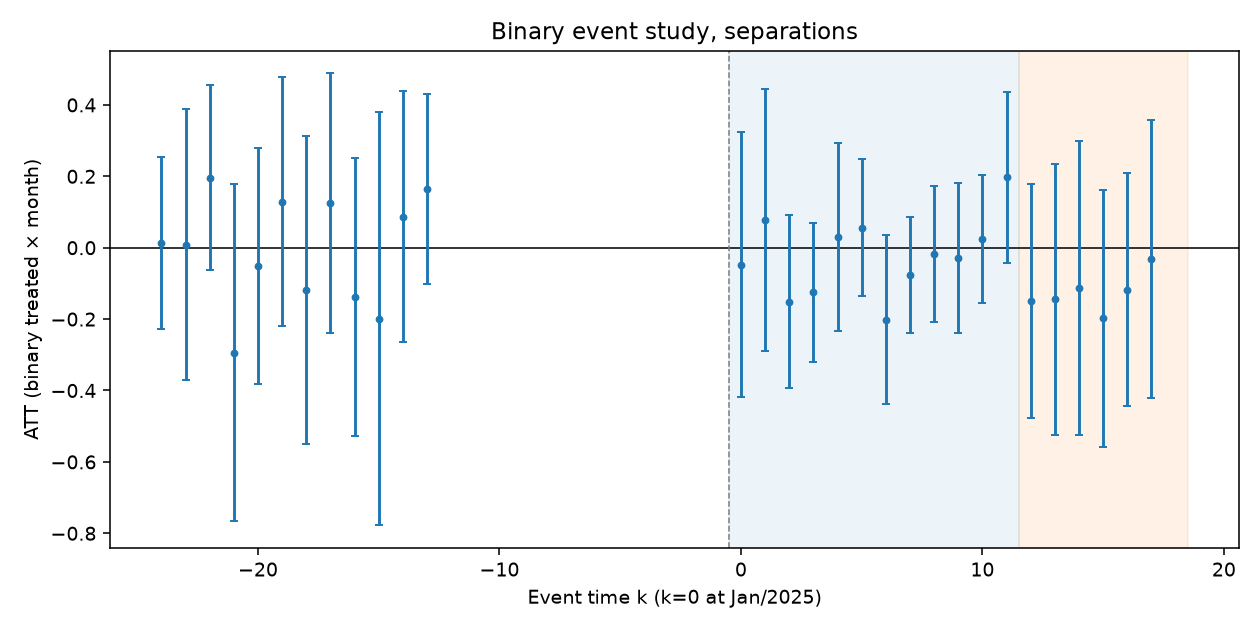
\includegraphics[width=0.95\textwidth]{fig_es_binario_base2024_desligados.png}
\caption{Binary ES for separations, principal specification. $T_{\max}$ $p\approx 0.42$.}
\label{fig:es_bin_des}
\end{figure}

\begin{figure}[H]
\centering
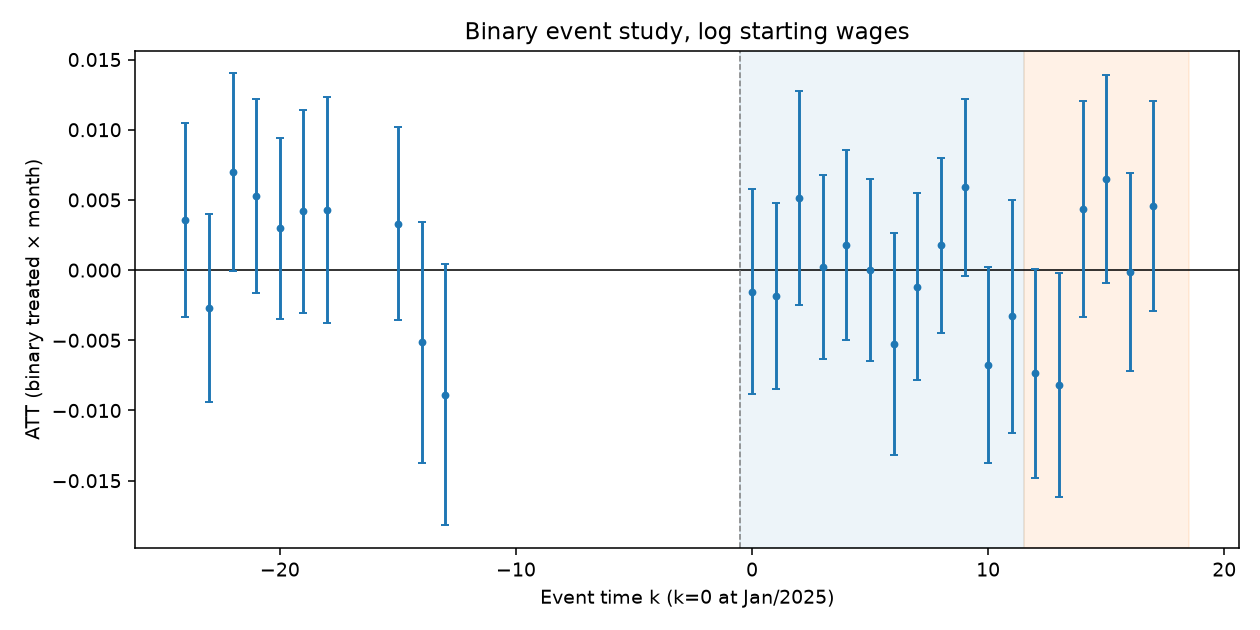
\includegraphics[width=0.95\textwidth]{fig_es_binario_base2024_log_salario.png}
\caption{Binary ES for log starting wages , principal specification. $T_{\max}$ $p\approx 0.41$.}
\label{fig:es_bin_wage}
\end{figure}

\section{Robustness sample cuts: supporting figures}
\label{app:es_rob}
% =====================================================================

Dose-$W$ event studies for hires, separations and log starting wages in the two sample cuts (without construction; CNAE-2 divisions with a listed class), principal specification. Net employment paths are in the body (Figures 5--6).

\begin{figure}[H]
\centering
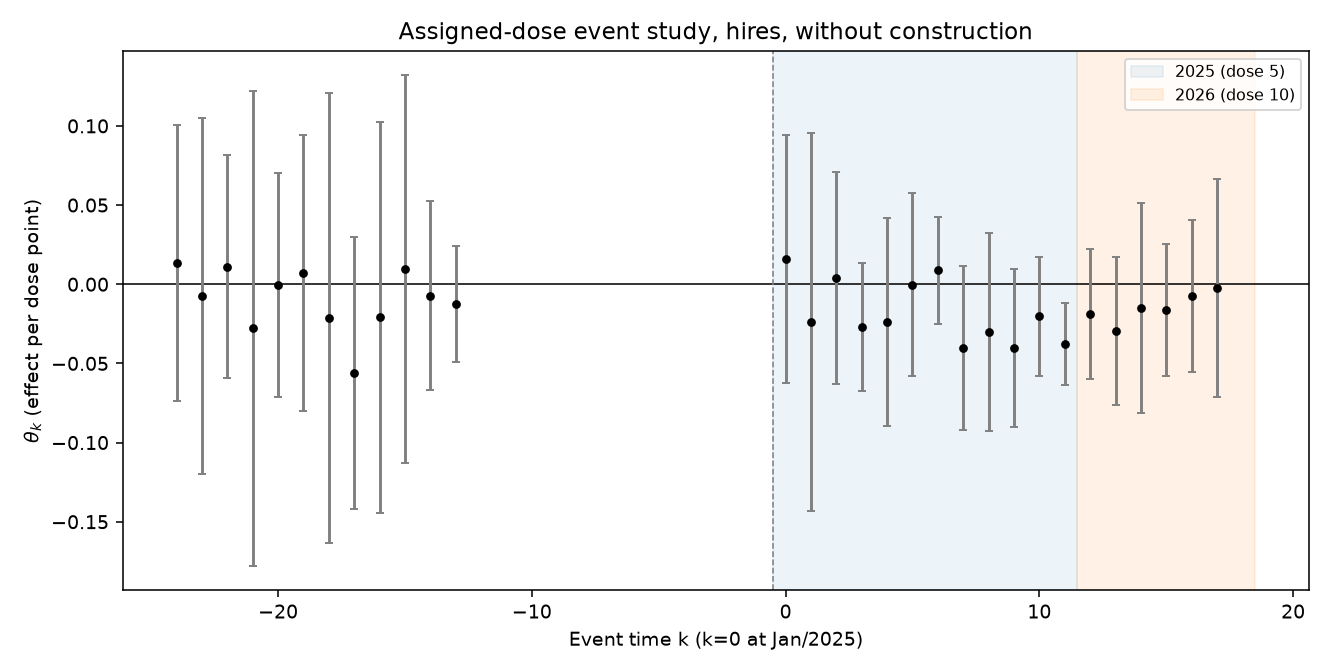
\includegraphics[width=0.95\textwidth]{fig_es_dose_semF_base2024_admitidos.png}
\caption{Dose-$W$ ES for hires, drop section~F, principal specification.}
\label{fig:es_dose_semF_adm}
\end{figure}

\begin{figure}[H]
\centering
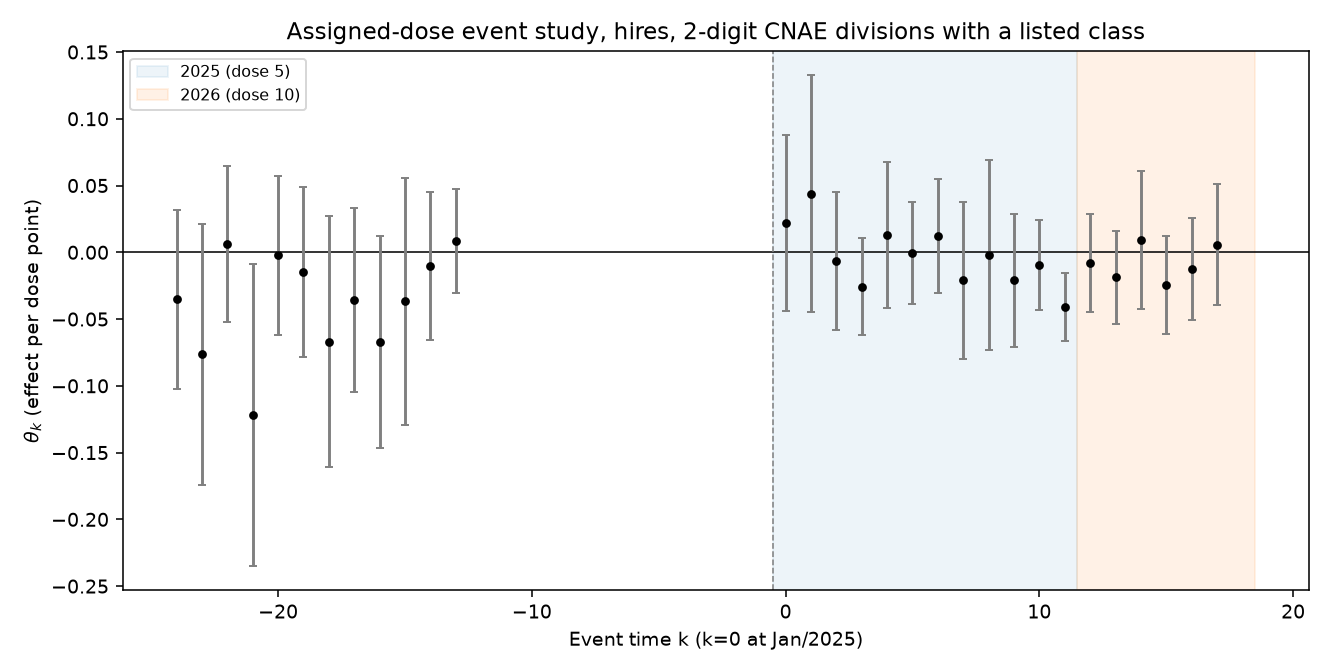
\includegraphics[width=0.95\textwidth]{fig_es_dose_cnae2_base2024_admitidos.png}
\caption{Dose-$W$ ES for hires, CNAE-2 with listed, principal specification.}
\label{fig:es_dose_CNAE-2_adm}
\end{figure}



\begin{figure}[H]
\centering
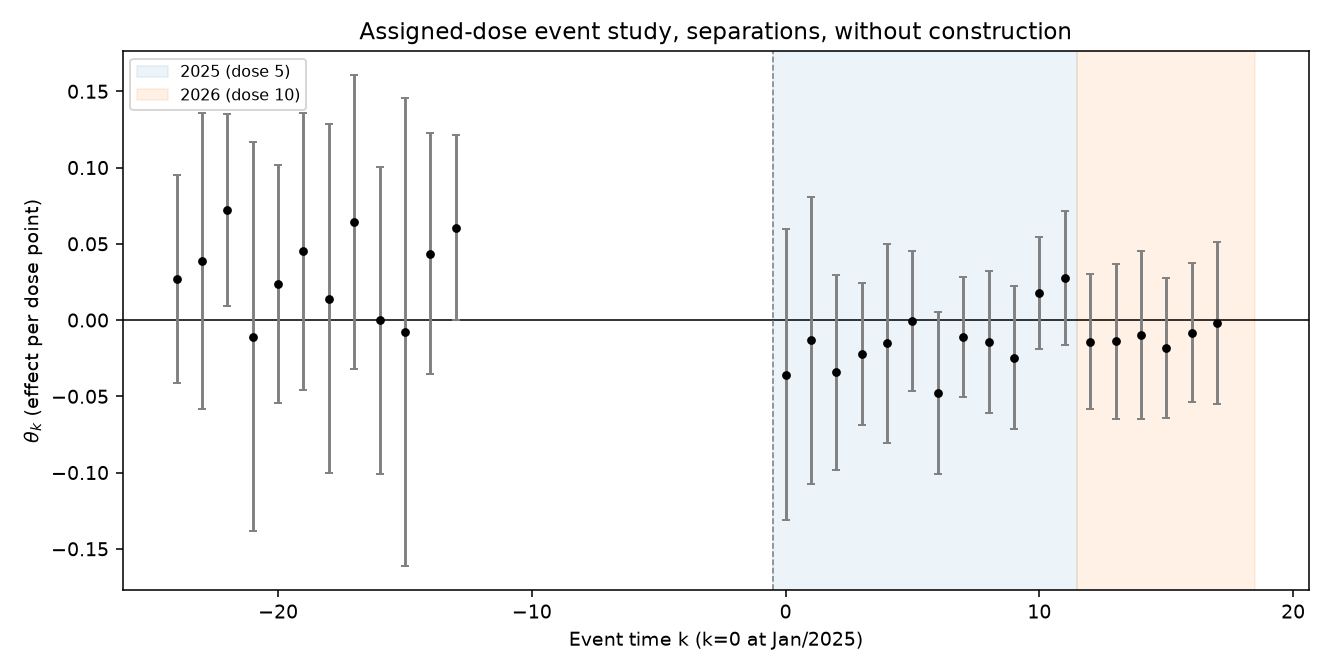
\includegraphics[width=0.95\textwidth]{fig_es_dose_semF_base2024_desligados.png}
\caption{Dose-$W$ event study for separations, drop section F, principal specification.}
\end{figure}

\begin{figure}[H]
\centering
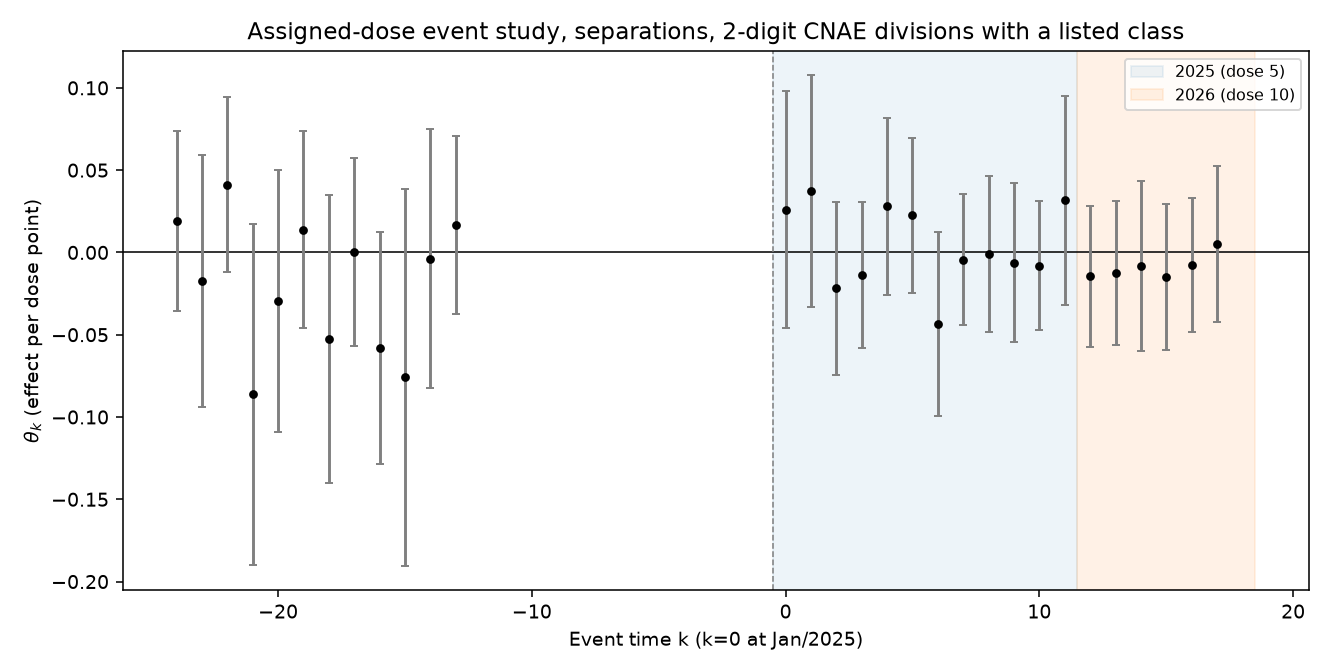
\includegraphics[width=0.95\textwidth]{fig_es_dose_cnae2_base2024_desligados.png}
\caption{Dose-$W$ event study for separations, CNAE-2 divisions with a listed class, principal specification.}
\end{figure}

\begin{figure}[H]
\centering
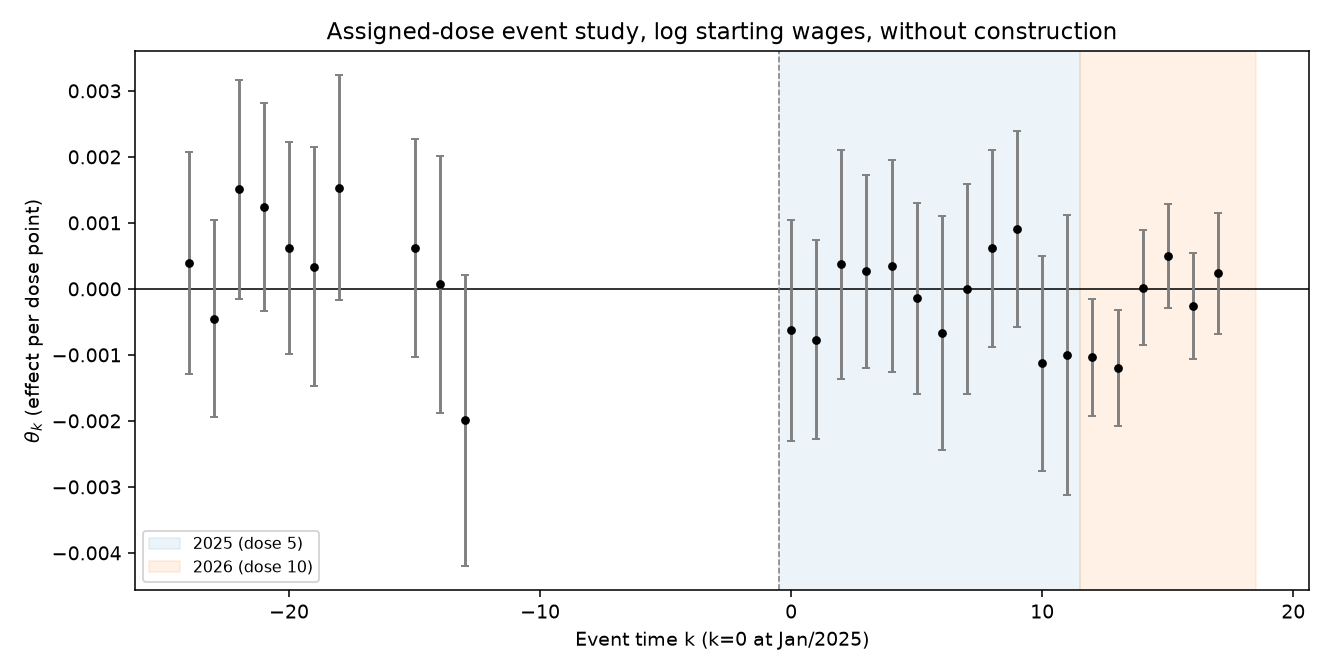
\includegraphics[width=0.95\textwidth]{fig_es_dose_semF_base2024_log_salario.png}
\caption{Dose-$W$ event study for log starting wages, drop section F, principal specification.}
\end{figure}

\begin{figure}[H]
\centering
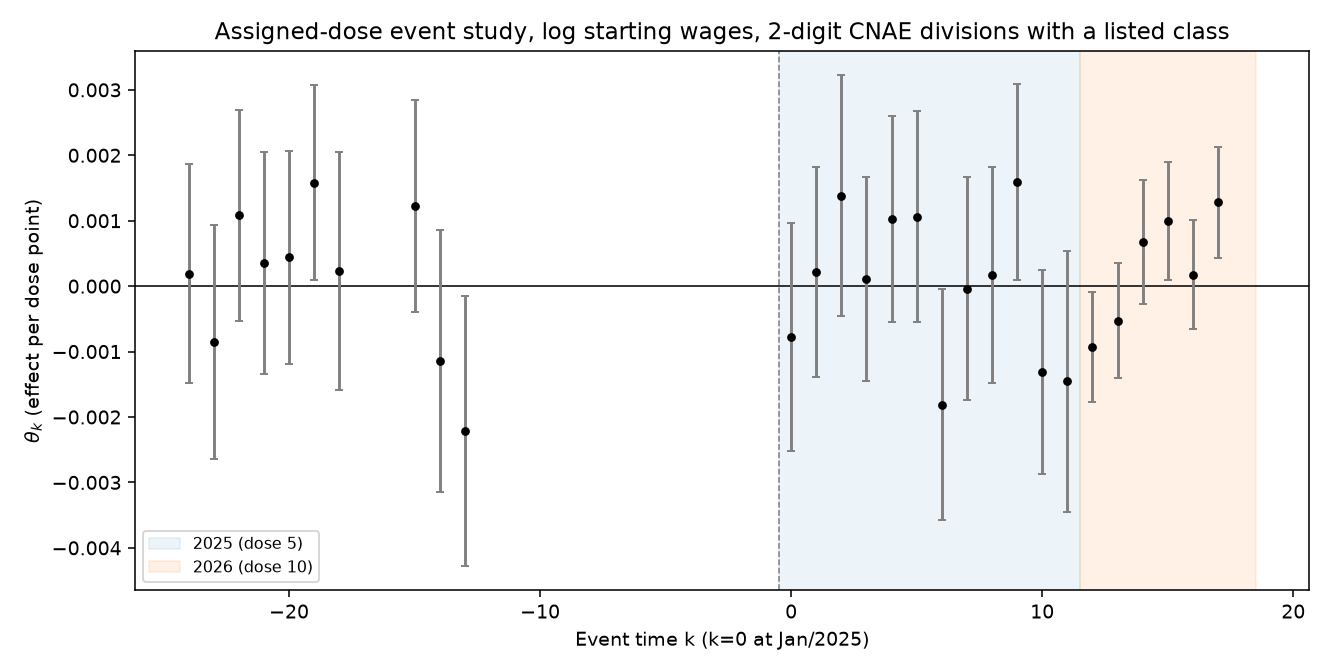
\includegraphics[width=0.95\textwidth]{fig_es_dose_cnae2_base2024_log_salario.png}
\caption{Dose-$W$ event study for log starting wages, CNAE-2 divisions with a listed class, principal specification.}
\end{figure}

\begin{thebibliography}{99}

\bibitem[Albernaz and Carvalho(2025)]{albernaz2025}
Albernaz, L.~R., and Carvalho, A.~X.~Y. (2025).
Desonera\c{c}\~ao e reonera\c{c}\~ao da folha de sal\'arios: efeitos sobre o emprego em setores beneficiados entre 2013 e 2018.
\textit{Revista Debates em Economia Aplicada}, 5(Único).
\url{https://www.portaldeperiodicos.idp.edu.br/redea/article/view/8808}.

\bibitem[Callaway et~al.(forthcoming)]{callaway2024}
Callaway, B., Goodman-Bacon, A., and Sant'Anna, P.~H.~C. (forthcoming).
Difference-in-differences with a continuous treatment.
\textit{American Economic Review}. doi:10.1257/aer.20240137.

\bibitem[de Chaisemartin and D'Haultf\oe uille(2020)]{de2022using}
de Chaisemartin, C., and D'Haultf\oe uille, X. (2020).
Two-way fixed effects estimators with heterogeneous treatment effects.
\textit{American Economic Review}, 110(9), 2964--2996.

\bibitem[Goodman-Bacon(2021)]{goodman2021using}
Goodman-Bacon, A. (2021).
Difference-in-differences with variation in treatment timing.
\textit{Journal of Econometrics}, 225(2), 254--277.

\bibitem[Montiel~Olea and Plagborg-M{\o}ller(2019)]{montiel2019}
Montiel~Olea, J.~L., and Plagborg-M{\o}ller, M. (2019).
Simultaneous confidence bands: Theory, implementation, and an application to SVARs.
\textit{Journal of Applied Econometrics}, 34(1), 1--17.

\bibitem[Reckziegel(2024)]{reckziegel2024}
Reckziegel, P.~H.~A. (2024).
\textit{Avaliação do impacto da política de desoneração da folha de pagamentos sobre o emprego}.
Dissertação de mestrado, Fundação Getulio Vargas, EBAPE.

\bibitem[Roth et~al.(2023)]{roth2023}
Roth, J., Sant'Anna, P.~H.~C., Bilinski, A., and Poe, J. (2023).
What's trending in difference-in-differences? A synthesis of the recent econometrics literature.
\textit{Journal of Econometrics}, 235(2), 2218--2244.

\end{thebibliography}
\end{document}
